\documentclass[a4paper,12pt]{article}

\usepackage[utf8]{inputenc}
\usepackage{listings}
\usepackage{color}
\usepackage{polski}
\usepackage[T1]{fontenc}

\usepackage{etoolbox}
\patchcmd{\thebibliography}{\section*{\refname}}{}{}{}
\usepackage{multicol}
\usepackage{biblatex}
\usepackage{pdfpages}

\usepackage{graphicx} 
\usepackage[export]{adjustbox}
\usepackage{wrapfig} 
\usepackage{subcaption}
\usepackage{amssymb}
\usepackage{setspace}
\usepackage{datetime}
\usepackage{mathptmx}
\usepackage{tocloft}
\usepackage{blindtext}
\usepackage{parskip}
\usepackage[hidelinks]{hyperref}
%
\definecolor{javared}{rgb}{0.6,0,0} % for strings
\definecolor{javagreen}{rgb}{0.25,0.5,0.35} % comments
\definecolor{javapurple}{rgb}{0.5,0,0.35} % keywords
\definecolor{javadocblue}{rgb}{0.25,0.35,0.75} % javadoc

\parskip=0.5\baselineskip \advance\parskip by 0pt plus 2pt


\lstdefinestyle{mystyle}{
    basicstyle=\linespread{1}\small\ttfamily,
    backgroundcolor=\color{white},   
    breakatwhitespace=false,         
    breaklines=false,                 
    captionpos=b,                    
    commentstyle=\color{javagreen},   
    escapeinside={\%*}{*)},          
    extendedchars=false,             
    keepspaces=true,                
    keywordstyle=\color{javapurple}\bfseries,
    morecomment=[s][\color{javadocblue}]{/**}{*/},
    language=Java,                
    numbers=left,                    
    numbersep=7pt,                  
    numberstyle=\tiny\color{black}, 
    rulecolor=\color{black},         
    showspaces=false,                
    showstringspaces=false,        
    showtabs=false,                  
    stepnumber=1,                  
    stringstyle=\color{javared},     
    tabsize=2,	                   
    title=\lstname,
    columns=flexible
}
%frame=single,	               
%basicstyle=\footnotesize,
\lstset{style=mystyle}

\urlstyle{
    colorlinks=true,
    linkcolor=blue,
    filecolor=magenta,      
    urlcolor=cyan,
    pdftitle={Sharelatex Example},
    bookmarks=true,
    pdfpagemode=FullScreen,
}

\newcommand{\MONTH}{%
  \ifcase\the\month
  \or Styczeń % 1
  \or Luty % 2
  \or Marzec % 3
  \or Kwiecień % 4
  \or Maj % 5
  \or Czerwiec % 6
  \or Lipiec % 7
  \or Sierpień % 8
  \or Wrzesień % 9
  \or Październik % 10
  \or Listopad % 11
  \or Grudzień % 12
  \fi
}
\makeatletter
\newcommand\spacingInSimpleItemize{0.8}
\newcommand\spacingInSolemnItemize{1.2}
\newcommand\spacingIndent{2.2em}
\newcommand\spacingVspace{0.7em}

\newcommand{\YEAR}{\@Roman{\the\year}}
\makeatother

\usepackage[left=2.5cm, right=2.5cm, top=2.5cm, bottom=2cm]{geometry}
\setlength{\parindent}{2.4em}
\setlength{\parskip}{1pt}
%\setlength{\parskip}{0.1\baselineskip plus2pt minus2pt}
\renewcommand{\baselinestretch}{1.5}
\renewcommand{\cftsecleader}{\cftdotfill{\cftdotsep}}
%?
\usepackage[11pt]{moresize}
\prefixing

\author{Przemysław Woldon}
\date{}

\begin{document}
    %strona tytułowa
    \begingroup
        \fontsize{12pt}{0.2}\selectfont
            \begin{center}Politechnika Łódzka\end{center}
            \begin{center}Wydział Elektrotechniki, Elektroniki, Informatyki i Automatyki\end{center} 
            \begin{center}Instytut Informatyki Stosowanej\end{center} 
        \vspace*{125px}     
        \fontsize{14pt}{0.2}\selectfont
            \begin{center}\textbf{PRACA DYPLOMOWA INŻYNIERSKA}\end{center} 
        \vspace*{50px}
        \fontsize{12pt}{0.2}\selectfont
            \begin{center}System umożliwiający digitalizację zapisów nutowych pieśni, \\\vspace{3mm} ułatwiający ich przechowywanie i przetwarzanie\end{center} \vspace{5mm}
            \begin{center}A system for digitization of sheet music facilitating their storage and processing\end{center} 
        \vspace*{50px}
        \fontsize{12pt}{0.2}\selectfont 
            \begin{center}Przemysław Woldon\end{center} 
            \begin{center}Numer albumu: 195092\end{center} 
        \vspace*{70px}
        \fontsize{12pt}{0.2}\selectfont 
            \begin{flushright}Opiekun pracy:\end{flushright} 
            \begin{flushright}Dr. inż. Paweł Kapusta\end{flushright} 
        \vspace*{185px}
        \fontsize{12pt}{0.2}\selectfont 
            \begin{center}Łódź, \MONTH \vspace{2cm}  \the\year \end{center} 
            \thispagestyle{empty}
    \endgroup
	\newpage
	
	\pagenumbering{gobble}
    \pagenumbering{arabic}
	\setcounter{page}{2}
	\begin{spacing}{1.35}
	%\begin{minipage}{\textwidth}
	    \noindent\begin{minipage}[s]{\textwidth}
            \tableofcontents
        \end{minipage}
    \end{spacing}
	\newpage 
	
\begin{spacing}{1.45}
\section*{Streszczenie}
	\addcontentsline{toc}{section}{Streszczenie}
	     \hspace{\spacingIndent} Niniejsza praca dyplomowa w sposób            zwięzły opisuje prototyp systemu umożliwiającego       pozyskanie tekstu z obrazów stron śpiewników kościelnych i     jego dalsze możliwości rozwoju. 
	     
         Na pracę pisemną składają się dwie zasadnicze części:        teoretyczna i praktyczna. Część teoretyczna opisuje           wybrane technologie, które zostały wykorzystane w             systemie. Wykorzystanym językiem programowania w którym powstała aplikacja był język Java, który determinował wybór frameworku dla sztucznych sieci neuronowych -- Deeplearning4J. Inne technologie które znalazły zastosowanie w systemie to OpenCV, wykorzystany do cyfrowego przetwarzania obrazów i system OCR Tesseract. Połączenie tych komponentów i zadbanie o ich właściwą współpracę umożliwiło prawidłowe działanie aplikacji. Część praktyczna w sposób przejrzysty           przedstawia szczegóły implementacyjne algorytmów. W podsumowaniu        autor w sposób krytyczny rekapituluje wykonaną pracę,          zwraca uwagę na zalety i wady wypracowanego                rozwiązania, jednocześnie podając sposoby na rozwiązanie      powstałych problemów oraz wskazuje drogi           rozwoju projektu.   
         
         Słowa kluczowe: Detekcja pięciolinii z partytur, OpenCV, Przetwarzanie obrazów, Konwolucyjne Sieci Neuronowe, Tesseract OCR.
	\section*{Abstract}
    \addcontentsline{toc}{section}{Abstract}   
    \hspace{\spacingIndent} This dissertation compactly describes the prototype of the system that allows obtaining text from images of church song pages and its further development possibilities.

    The thesis contains two major part: practical and theoretical.
    The theoretical part describes the selected technologies which 
    were used in system. Java was the utilized programing language which 
    determined choice of framework for artificial neural networks - Deeplearning4J. Other technologies which are used in system: OpenCV, which was used for digital image processing and Tesseract OCR system. The combination of these components and ensuring their appropriate cooperation enabled the correct operation of application. The practical part introduces implementation details of algorithm in a transparent way. In the summary, author recapitulates executed work executed in a critical way, notes advantages and disadvantages of elaborated system, at the same time author hands ways to solve existing problems and opportunities of the development of the system.
    
    Keywords: Music sheet detection, OpenCV, Image Processing, Convolutional Neutral Network, Tesseract OCR.
    \end{spacing}
	
	\newpage 
	\noindent\begin{minipage}[s]{\textwidth}
	\section{Wstęp}
		\hspace{\spacingIndent} Informatyzacja dotyka wielu obszarów naszego       życia. Jednym z nich jest sztuka (w tym muzyka, muzyka        sakralna). Obecnie coraz częściej w świątyniach możemy        spotkać się z rzutnikami lub wyświetlaczami LED, 
			na których ekranizowane są teksty pieśni. Cyfrowe zbiory pieśni dostarczane przez producentów wyświetlaczy 
			nie są w stanie sprostać wymaganiom jakie stawia przed nimi: dynamiczny rozwój muzyki -- powstawaniu nowych utworów, 
			zróżnicowanym tradycjom lokalnym oraz indywidualnym upodobaniom muzyków kościelnych wykorzystującym różne śpiewniki. 
			Czasochłonny proces budowy wspomnianych zbiorów często polega na ręcznym przepisywaniu tekstów pieśni 
			z wykorzystywanych przez muzyków kościelnych śpiewników. Automatyzacja tego procesu pozwoli na łatwiejsze dopasowanie zbiorów 
			do potrzeb muzyków kościelnych i tradycji lokalnych. 
	        Przed przystąpieniem do prac nad aplikacją autor nie      spotkał się z wykorzystaniem na rynku polskim             oprogramowania rozwiązującego powyższe problemy.
		
		 \hspace{\spacingIndent} Dzięki pracy nad tą aplikacją autor mógł połączyć swoje dwie pasje -- muzykę kościelną i informatykę. 
			Pomysł budowy aplikacji narodził się z zaobserwowania, że osoby odpowiedzialne za muzykę kościelna przeznaczają znaczącą liczbę godzin 
			na ręczne przepisywanie śpiewników, poprawę błędów w już dostarczonych zbiorach. Zaangażowanie technik informatycznych do tego zadania 
	        umożliwi szybszą budowę własnych zbiorów pieśni.  
			Budowa prototypu zapewniającego pełną funkcjonalność,  daje możliwość jego opublikowania 
			i dotarcia do szerokiego grona interesariuszy, co może stanowić punkt wyjściowy do dalszych prac nad aplikacją tak aby wypracowane rozwiązanie było użyteczne, niezawodne, wydajne i wspierane.
		
		\subsection{Cel pracy}
			\hspace{\spacingIndent} Celem niniejszej pracy dyplomowej było skonstruowanie algorytmów przetwarzających strony śpiewników kościelnych tak, 
				aby jak najlepiej przygotować je do optycznego rozpoznania zawartego w nich tekstu. W algorytmach wykorzystane zostały metody przetwarzania obrazów, 
				które redukują szumy, usuwają obszary, które nie zawierają znaczących w analizie danych (eliminacja nadmiarowych informacji), 
				prostują strony, wykrywają i usuwają znaki muzyczne, wykrywają znaki (cyfry, litery, znaki interpunkcyjne), 
				zaś algorytmy cyfrowego rozpoznawania tekstu odczytują wykryte litery uwzględniając polskie znaki diakrytyczne. 
				Dzięki zastosowaniu konwolucyjnych sieci neuronowych wypracowane rozwiązanie zostało uogólnione, a \nopagebreak finalne algorytmy umożliwiają pracę 
				na różnych danych wejściowych. Zaś budowa aplikacji uwzględniająca dobre praktyki programowania ułatwi jej dalszy rozwój.
				
		\end{minipage}
				
	\newpage 

	\section{Wykorzystane technologie}
	    \hspace{\spacingIndent} Założenia początkowe, które miał spełnić system możliwe były do osiągnięcia przy wykorzystaniu różnych technologii dostępnych na rynku. Wybrane zostały następujące narzędzia: do przetwarzania obrazów -- biblioteka OpenCV, do budowy sztucznych sieci neuronowych -- DL4J, do odczytania tekstu -- Tesseract, zaś całość została napisana w języku programowania Java. Właściwe połączenie i wykorzystanie tych elementów pozwoliło na zrealizowanie założeń systemu. Technologie te zostały opisane w kolejnych podrozdziałach wraz z ich zaletami, które zadecydowały o ich wyborze.
	    
		\subsection{Biblioteka OpenCV}
		\hspace{\spacingIndent} Cyfrowe przetwarzanie obrazów \textit{(ang. digital image processing)} jest dziedziną nauki 
			zajmującą się reprezentacją obrazu w pamięci komputera, jego akwizycją i przetwarzaniem. 
         Obecnie dostępnych jest wiele bibliotek umożliwiających pracę z obrazami, na przykład: Imagemagick, Generic Image Library, SIMD i inne. 
			Najbardziej powszechną biblioteką jest jednak biblioteka OpenCV. Wieloletnia praca nad algorytmami przetwarzającymi obrazy pozwoliła zbudować optymalną i bardzo bogatą, bezkonkurencyjną funkcjonalność.
			Ponadto OpenCV posiada przejrzystą 
			i zawierającą podstawy matematyczne dokumentację, zaś dynamicznie rozwijająca się społeczność zgromadzona wokół biblioteki ułatwia 
			z nią pracę szczególnie nowym użytkownikom.
			%\paragraph{\indent} 
			%	OpenCV jest biblioteką służącą do komputerowego przetwarzania obrazów oraz uczenia maszynowego, o otwartym kodzie źródłowym.
		\subsubsection{Zarys historyczny}
			\hspace{\spacingIndent} Prace nad budową tej biblioteki rozpoczął jeden z pracowników firmy Intel -- Gary Rost Bradski, 
				zainspirowany środowiskiem akademickim, które wówczas posiadało bardzo bogatą infrastrukturę służącą do przetwarzania obrazów, 
				jednak przeznaczoną dla użytku wewnętrznego. Studenci w obrębie jednej jednostki akademickiej dzielili się kodem zawierającym gotowe 
				implementacje algorytmów, co znacząco ułatwiało prace przy własnych projektach czy aplikacjach. Stąd głównym celem biblioteki OpenCV 
				jest udostępnienie wszystkim zainteresowanym zagadnieniami przetwarzania obrazów i sztucznej inteligencji gotowej, jednolitej, 
				darmowej infrastruktury pozwalającej na pracę, tak aby nie trzeba było ponownie "wynajdywać koła" \cite{3}. 
				
			OpenCV zostało przedstawione po raz pierwszy w 1999 roku szerszemu gronu odbiorców.  W wersji 1.0 kod biblioteki stanowiły wyłącznie najbardziej użyteczne przy przetwarzaniu obrazów algorytmy zaimplementowane w języku C. 
				Od tego czasu biblioteka znacząco się zmieniła. 
			
			 W wersji 2.0 znaczący wpływ na wydanie wywarły trendy obecne w prowadzeniu projektów, w których wytwarza się oprogramowanie -- repozytorium kodu
				w systemie kontroli wersji Git, gdzie możemy znaleźć najnowszą wersję biblioteki i najświeższe poprawki, testy jednostkowe czy booty ciągłej kompilacji. 
				Zaimplementowano również interfejsy dla języków programowania takich jak C++ oraz Javy, Python’a, MATLAB--a. Od tego czasu nowe typy danych 
				i funkcje metody implementowano w C++, a już napisane w języku C dopasowano do nowej technologii. 
			
			Nieustannie zwiększająca się liczba zaimplementowanych algorytmów użytecznych przy przetwarzaniu obrazów przyczyniła się do modułowej budowy 
				biblioteki w wersji 3.0, wspiera ona budowanie i dołączanie do biblioteki własnych modułów, przedstawia się ona w sposób następujący:
                
                \begin{spacing}{\spacingInSolemnItemize}
    				\begin{itemize}
    					\item (warstwa wierzchnia) system operacyjny,
    					\item interfejsy dla różnych języków i aplikacje,
    					
    					
    					\item moduł \textit {opencv\_contrib} zawierający kod napisany i dołączony do biblioteki przez użytkowników,
    					\item rdzeń OpenCV,
    					\item optymalizacje sprzętowe (warstwa HAL \textit {ang. hardware acceleration layer}).
    				\end{itemize} 
                \end{spacing}
            
				\begin{figure}[!ht]  
					\begin{center}
						\includegraphics[width=12cm] {image//openCvBudowa.png} 
					\end{center}
					\caption
					    [Budowa modułowa OpenCV]
					    {Budowa modułowa OpenCV}
				\end{figure}

				 
	            \newpage
				\begin{figure}[!ht]   
					\begin{center}
		    				\includegraphics[width=\linewidth] {image//osCzasu.png} 
					\end{center}
					\caption
					    [Rozwój projektu w czasie]  
					    {Rozwój projektu w czasie}  
				\end{figure}


		\subsubsection{Popularność projektu}  
			\hspace{\spacingIndent} Projekt cieszy się bardzo dużym powodzeniem, które nieustannie rośnie. Świadczy o tym liczba pobrań 
				wynosząca około 14 milionów razy, zaś miesięcznie około 200 tysięcy. Obecnie biblioteka zawiera ponad 2500 zoptymalizowanych algorytmów, 
				które służą do przetwarzania obrazów również w czasie rzeczywistym i uczenia maszynowego, co znacząco ułatwia tworzenie aplikacji użytkownikom. 
				Programiści piszący kod uwzględniali wymóg przenośności OpenCV, a więc możliwości kompilacji na każdym odpowiednim kompilatorze języka C++, 
				co wymusiło restrykcyjną zgodność ze standardem i ułatwiło obsługę różnych platform. Biblioteka dostępna jest na systemach operacyjnych takich jak: 
				Windows, Linux, Mac OS X, do których dołączyły systemy operacyjne platform mobilnych (Android i iOS), co znacząco przyczyniło się do zwiększenia liczby użytkowników.

		\subsubsection{Zastosowania biblioteki OpenCV}
			\hspace{\spacingIndent} Dynamiczny rozwój technologiczny otwiera przed biblioteką nowy horyzont użyteczności. 
				OpenCV znajduje zastosowanie w wielu obszarach życia do tego stopnia że wykorzystanie projektu wydaje się rzeczą całkowicie naturalna,
				a wręcz niezauważalną. Biblioteka wykorzystywana jest w:
			
			    \begin{spacing}{\spacingInSolemnItemize}
			        \begin{itemize}
        				\item skanowaniu kodów QR,
        				\item monitoringu,
        				\item rozpoznawaniu dźwięków i muzyki,
        				\item obrazowaniu medycznym,
        				\item robotyce,	
        				\item przemyśle -- produkcji masowej i kontroli jakości,
        				\item wojsku -- bezzałogowe pojazdy, fotografie lotnicze,
				        \item analizie obiektów,
				        \item Google Street View
		            \end{itemize}
                \end{spacing}
    
    	\subsubsection{Reprezentacja obrazów}
			\hspace{\spacingIndent} Obrazy można podzielić w najprostszy sposób na obrazy barwne i obrazy w skali szarości. Obrazy w bibliotece OpenCV 
				reprezentowane są w postaci macierzy \textit{(Mat)}. Narzędzie to udostępnia bogatą gamę możliwości reprezentacji poszczególnego piksela, 
				a więc i samego obrazu. Tak więc jeden piksel jest reprezentowany w następujący sposób -- CV\_xCy, gdzie:
			
				\begin{spacing}{\spacingInSolemnItemize}
					\begin{itemize}
						\item{x -- parametr określający typ}
							\begin{itemize}
								\item{8U -- 8-bitowy char bez znaku}
								\item{16S -- 16-bitowy short ze znakiem}
								\item{16U -- 16-bitowy short bez znaku}
								\item{32S -- 32-bitowa liczba całkowita ze znakiem}
								\item{32F -- 32-bitowa liczba zmiennoprzecinkowa}
								\item{64F -- 64-bitowa liczba zmiennoprzecinkowa}
							\end{itemize}
						\item{y  -- parametr określający liczbę kanałów}
							\begin{itemize}
								\item{1 -- jeden kanał}
								\item{2 -- dwa kanały}
								\item{3 -- trzy kanały}
							\end{itemize}
					\end{itemize}	
				\end{spacing} Jeśli użytkownik potrzebuje więcej kanałów może użyć funkcji CV\_xC(n), gdzie n -- liczba kanałów. Można również wybierać 
				z obfitej przestrzeni reprezentacji obrazu np. RGB, RGBA, HSV i innych. 
			
			 Obrazy przechowywane jako pliki w pamięci komputera mają różne rozszerzenia, które wpływają na ich jakość, 
				wielkość zajmowanego miejsca na dysku. Przykładowe formaty obrazów: 
			
				\begin{spacing}{\spacingInSolemnItemize}
					\begin{itemize}
						\item TIFF \textit{(ang. Tagged--lmage File Format)} -- format standardowy i najbardziej podstawowy, używa algorytmu kompresji bezstratnej;
						\item JPEG \textit{(ang. Joint Photographic Experts Group)} -- używa algorytmu kompresji stratnej;
						\item PNG \textit{(ang. Portable Network Graphics)} -- używa algorytmu kompresji bezstratnej; 
						\item GIF \textit{(ang. Graphics Interchange Format)} -- używa algorytmu kompresji bezstratnej LZW \textit{(Lemple-Zif-Welch)}, 
							pliki mają małe rozmiary, często jest wykorzystywany do tworzenia animacji;
					\end{itemize}
				\end{spacing}
    
    \subsection{Konwolucyjne sieci neuronowe}
        \hspace{\spacingIndent} Działanie sztucznych sieci neuronowych \textit{(Artificial neural network (ANN))} opiera się na modelu pojedynczego     
			neuronu (perceptronu), które zostają łączone w większe struktury. Matematyczną podstawę dla działania konwolucyjnych sieci neuronowych 
			\textit{(Convolutional neural networks (CNN))} stanowi splot (konwolucja) -- jest to operacja określana na dwóch funkcjach (np. f(t), g(t)) 
			w wyniku której otrzymujemy nową funkcję (np. h(t)); w przetwarzaniu obrazów jedną z funkcji jest analizowany obraz wejściowy, zaś druga filtr.
            Obraz wejściowy przechodzi przez wiele filtrów i każdy z nich mapuje cały obraz wejściowy biorąc pod uwagę jego części o rozmiarze filtra. 
			Tak wiec konwolucyjne sieci neuronowe uczą się obrazu, analizując go pewnymi wycinkami. Dokładnie filtr przechodzący przez obraz 
			mnoży odpowiednie wartości a następnie sumuje ich iloczyny.
			
			
        
            \begin{displaymath}
                h[m, n] = ( f \star g)[m, n] = \sum\limits_{j}\sum\limits_{k}f[j, k]g[m-j, n-k]
            \end{displaymath}
            
            Przykład działania konwolucji został zaprezentowany na Rysunku \ref{fig:przykladDzialaniaKonwolucji}. 
            Przez każdy z kanałów obrazu wejściowego (kolor niebieski) przechodzą dwa filtry (kolor czerwony). Krok z jakim filtr przesuwa się wynosi dwa piksele (dwie kolumny) co można zaobserwować na parze (a) i (b) oraz parze (c) i (d). Wynik działania każdego z filtrów zapisywany jest do macierzy wynikowej (kolor zielonego). 
            
            %Obraz wejściowy (koloru niebieskiego), który jest trójkanałowy zostaje przetworzony przez dwa filtry (koloru czerwonego), które przesuwają się co 2 piksele (dwie kolumny), przechodzą przez obraz wejściowy , a wynik działania splotu zostaje zapisany w macierzy wynikowej (koloru zielonego).
            
		    \newpage
		    
    	    \begin{figure}[h!]
                \centering
                \begin{subfigure}[b]{0.47\linewidth}
                    \includegraphics[width=\linewidth]{image//con_01.png}
					\caption{}
                \end{subfigure}
                \begin{subfigure}[b]{0.47\linewidth}
                     \includegraphics[width=\linewidth]{image//con_02.png}
					\caption{}
                \end{subfigure}
                \newline
                
				\begin{subfigure}[b]{0.47\linewidth}
                    \includegraphics[width=\linewidth]{image//con_03.png}
					\caption{}
                \end{subfigure}
                \begin{subfigure}[b]{0.47\linewidth}
                    \includegraphics[width=\linewidth]{image//con_04.png}
					\caption{}
                \end{subfigure}
                \caption
                    [Przykład działania konwolucji]
					{Przykład działania konwolucji \\  Źródło: \href{https://skymind.ai//wiki//convolutional-network}{\url{https://skymind.ai//wiki//convolutional-network}}, 
					data dostępu: 09.07.2018}
					\label{fig:przykladDzialaniaKonwolucji}
            \end{figure}
        
			Następnie dane wejściowe przechodzą przez nieliniową transformację (funkcję aktywacji), która określa czy perceptron będzie aktywowany czy nie. 
			Funkcja ta odgrywa znacząca rolę w dopasowaniu gradientów. Funkcje te są ciągłe i różniczkowalne (wyjątek stanowi funkcja ReLU w zerze).
        
			Wśród funkcji aktywacji wyróżniamy funkcje takie jak: funkcja sigmoidalna,  tangens hiperboliczny \textit{(tanh)}, które mapują wartość wejściowa w zakresach odpowiednio (0, 1), (-1, 1). 
			Bardzo duża popularnością dla warstw ukrytych sieci neuronowej cieszy się funkcja aktywacji: rektyfikowana jednostka liniowa 
			\textit{(ang. The Rectified Linear Unit (ReLU))}, która jest najprostszą nieliniową funkcją aktywacji. Prostota tego rozwiązania niesie ze sobą również pewne niebezpieczeństwo całkowitego wykluczenia neuronu (neuron nigdy nie będzie aktywowany) przy zbyt szybkim uczeniu się sieci.
			Sama funkcja przyjmuje wartość zero dla wartości mniejszych od zera i wartość wejścia jeśli jest ono większe lub równe zero.
			
			\begin{displaymath}
			%\begin{equation}
                f(x) =  
                \left\{
                    \begin{array}{ll}
                        0 & \textrm{dla } x < 0 \\
                        x & \textrm{dla } x \geqslant 0
                    \end{array}
                \right.
                %\label{eq:relu}
            %\end{equation}
            \end{displaymath}
			Funkcja softmax przetwarza wektor wejściowy na wektor wyjściowy według następującego wzoru będącego rozkładem prawdopodobieństwa, 
			mówiącego o prawdopodobieństwie wystąpienia poszczególnej klasy \cite{13}. 
        \begin{center}
			\begin{displaymath}
				\sigma (z)_{j} = \frac{e^{z_{j}}}{ \sum_{k=1}^K e^{z_{j}}}
			\end{displaymath}
			\end{center}
			Suma wartości wektora wyjściowego wynosi jeden. Wektor wejściowy oraz wyjściowy mają taki sam rozmiar. Funkcja normalizuje K wymiarowy wektor w K wymiarowy wektor  
			$ \sigma (z)$. 
        
	    Zjawiskiem występującym przy zastosowaniu konwolucyjnych sieci neuronowych jest pooling (Rysunek \ref{fig:maxPooling}). Polega on na zmniejszeniu wymiarowości 
			przetwarzanego obrazu. Zaletą zastosowania poolingu jest wyeksponowanie znaczących informacji, które zawiera obraz. Można wyróżnić average 
			pooling i max pooling i inne. Pooling może być wykonany na każdym z kanałów obrazu z różnym rozmiarem jądra oraz różnym krokiem. 
	 
			\begin{figure}[!ht]
				\centering
				\includegraphics[width=17cm, height=4.5cm]{image//maxPoolingImg.png}
				\caption
				[Max pooling]
				{Max pooling}
				\label{fig:maxPooling}
			\end{figure}
        
			Pooling jest również metodą regularyzacji sieci neuronowej, zapobiegający jej przeuczeniu. Algorytmy służące regularyzacji stosuje się, aby sieć lepiej klasyfikowała dane testowe. Dzięki różnym techniką regularyzacji zmniejszany jest błąd generalizacji sieci neuronowej (jednak nie błąd szkoleniowy). 
        
        Inną efektywną drogą regularyzacji sieci neuronowych również zapobiegającą zjawisku przeuczenia się sieci jest dropout. 
			Podczas treningu sieci zostają wykluczone, dezaktywowane nadmiarowe neurony z architektury sieci w sposób losowy, 
			w efekcie może on uwzględniać np. neurony o najmniejszych wagach, które nie mają większego wpływu na ostateczny wynik działania sieci. 
			Tak odrzucone neurony nie biorą już udziału w końcowym procesie wnioskowania. Obok dropout'u istnieją takie metody zapobiegające 
			przeuczeniu się sieci jak: legularyzacja l1 i l2, zmniejszające wartość absolutną, pierwiastek kwadratowy wag, uznając, że modele mające 
			zminimalizowane wagi osiągają lepsze wyniki. Regularyzacja, a w szczególności dropout pozytywnie wpływa na minimalizację błędu 
			klasyfikacji sieci neuronowej \cite{15}. 
        
        Zasadniczym metodą bez której uczenie się sieci neuronowych byłoby niemożliwe, a której implementacje jednocześnie służą optymalizacji sieci neuronowych (wielowarstwowych) jest algorytm wstecznej propagacji błędów 
			\textit{(ang. backpropagation)}. Wagi poszczególnych połączeń mogą zostać wytrenowane, a więc dobrane automatycznie i stanowiące 
			w przybliżeniu zestaw najbardziej optymalny. Wsteczna propagacja błędów polega na aktualizowaniu wartości wag na podstawie wartości błędu 
			wag dotychczasowych. W celu poprawy efektywności wstecznej propagacji błędów często zaleca się następujące metody: 
			zastosowanie losowych wag początkowych, kilkukrotne powtarzanie procesu uczenia. Sam algorytm uwzględnia następujące kroki 
			zakładając losową generację wag początkowych: obliczenie odpowiedź sieci dla każdego z wektorów uczących, 
			każdy z neuronów wyjściowych oblicza swój błąd, propagacja błędów do warstw wcześniejszych, na podstawie propagowanej wartości 
			błędu każdy z neuronów modyfikuje wagi, powyższe kroki są powtarzane dopóki średni błąd nie przestanie maleć.
\subsubsection {Sieci konwolucyjne w języku Java}
        \hspace{\spacingIndent} Do budowy konwolucyjnych sieci neuronowych został wykorzystany framework Deeplearning4j. Działa on na wirtualnej maszynie Javy. 
			Można go wykorzystywać z językiem programowania Java (DL4J) i Scala (DL4S). Narzędzie posiada bogatą dokumentacje, repozytorium kodu na 
			platformie GitHub gdzie znajdują się zaimplementowane gotowe przykłady użycia frameworku 
			\href{https://github.com//deeplearning4j//nd4j}{\url{https://github.com//deeplearning4j//nd4j}}. Umożliwia konfigurację środowiska 
			za pośrednictwem narzędzi automatyzujących budowę projektu, na przykład: Maven, Gradle, Ivy, SBT. Do operacji backendowych narzędzie 
			udostępnia wybór pomiędzy GPU, a CPU. Framework posiada zaimplementowane mechanizmy budowy, regularyzacji, optymalizacji sieci neuronowych, 
			różnorodne rodzaje warstw z których możemy budować architekturę sieci (główne grupy) : Feed-Forward Layers, Output Layers, Convolutional Layers, 
			Recurrent Layers,  Unsupervised Layers, Other Layers, Graph Vertices, InputPreProcessors. 
			W pracy wykorzystywane są następujące z udostępnionych warstw wraz z konfiguracją: 

			\begin{spacing}{\spacingInSolemnItemize}
				\begin{itemize}
					\item \textit{ConvolutionLayer} -- warstwa wykonująca konwolucję
						\begin{itemize}
							\item \textit{ConvolutionLayer.Builder(x, y)} -- określa wielkość jądra; \textit{x} -- jego szerokość w pikselach, a \textit{y} -- jego wysokość w pikselach,
							\item \textit{stride(m, n)} -- określa krok z jakim jądro jest przesuwane na obrazie wejściowym; \textit{m} -- przesunięcie na osi odciętych w pikselach, 
								a \textit{n} -- przesunięcie na osi odciętych w pikselach,
							\item \textit{nOut(k)} -- określa liczbę filtrów przez które przechodzi obraz;
						\end{itemize}
				% 		\newline 
				% 		\vspace*{15px}
					\item \textit{SubsamplingLayer} -- warstwa odpowiadająca za pooling,
						\begin{itemize}
							\item \textit{SubsamplingLayer.Builder(SubsamplingLayer.PoolingType.n)} -- \textit{n} -- określa rodzaj poolingu z pośród: MAX, AVG, SUM, PNORM; 
							\item \textit{kernelSize(m, n)} -- określa wielkość jądra; \textit{m} -- jego szerokość w pikselach, a \textit{n} -- jego wysokość w pikselach,
						\end{itemize}
					\item \textit{DenseLayer} -- warstwa standardowa biorąca pod uwagę wszystkie wyjścia z warstwy poprzedniej,
					\item \textit{OutputLayer} -- warstwa wyjściowa odpowiadająca za klasyfikację;
				\end{itemize}
			\end{spacing}
			\vspace{\spacingVspace}
		 Narzędzie wspiera następujące parametry konfiguracji sieci lub poszczególnych warstw (Listing \ref{lst:przykladowaSiec}) : funkcja aktywacji , inicjalizacja wag początkowych, 
			aktualizacje kroku uczenia, regularyzację i inne. Wszystkie dostępne warstwy i parametry konfiguracji sieci dostępne są na stronie projektu:
			\href{https://deeplearning4j.org//quickref\#config}{\url{https://deeplearning4j.org//quickref\#config}}.
			\newline
            \lstinputlisting[caption={Przykładowa konfiguracja konwolucyjnej sieci neuronowej},label={lst:przykladowaSiec}]{przykladowaSiec.java}
		
        
        
	\subsection{Tesseract OCR}
	    \hspace{\spacingIndent} Tesseract jest systemem służącym do optycznego rozpoznawania znaków (OCR \textit{ang. optical character recognition}) 
			opracowanym przez firmę HP, obecnie projekt jest sponsorowany przez Google. System został napisany w języku C. 
			Dostępne są interfejsy umożliwiające korzystanie z narzędzia, z poziomu innych języków np. Java (wrapper Tess4J). 
			
			 Pierwsza wersja umożliwiała pracę z językiem angielskim, kolejne wydania powiększały listę pakietów językowych, 
			najpierw o inne języki zachodnioeuropejskie, a później o inne języki używane w świecie. Na szczególna uwagę wśród nich zasługują japoński, chiński, 
			i języki semickie czytane od prawej do lewej. Obecne narzędzie udostępnia wybór pakietu językowego uwzględniającego 
			znaki diakrytyczne wśród około 130 możliwych. Oprócz obsługi różnych języków możliwa jest obsługa różnych czcionek. 
			
			W początkowej wersji Tesseract pozwalał na pracę z plikami o rozszerzeniu TIFF. Kolejne wersje systemu umożliwiają pracę z bogatszą gamą plików: 
			JPEG, GIF, PNG, BMP, wielostronicowych plików TIFF dzięki wykorzystaniu biblioteki służącej do przetwarzania obrazów -- Leptonica 
			(wrapper Java -- Lept4J). Dzięki współpracy dodatkowych bibliotek (GPL Ghostscript lub PDFBox) możemy odczytywać tekst zawarty w plikach PDF.			Dodatkowymi funkcjonalnościami, które zasługują na uwagę są: możliwość analizy układu strony, uzyskania informacji o położeniu rozpoznanego tekstu na stronie 
			i formatowanie tekstu wyjściowego. 
			
			Projekt dostępny jest na wielu platformach: Windows, Linux, Mac OS X. Tesseract nie udostępnia graficznego interfejsu użytkownika, 
			a sama konfiguracja systemu i przetwarzanie danych odbywa się z poziomu konsoli, powstały jednak systemy wykorzystujące tesseracta i posiadające GUI. 
			
			Oprogramowanie w pewnych okolicznościach jest wrażliwe na błędy, należy unikać rozmiaru tekstu mniejszego niż 20px, pochylonego lub obróconego, 
			niepozytywnie na działanie wpływają również ciemne granice strony ponieważ mogą one zostać rozpoznane i dopasowane jako znaki. Mimo to silnik Tesseracta uznawany jest za jeden z najlepiej działających wśród dostępnych systemów OCR. 

	\subsection{Środowisko programistyczne}
		\hspace{\spacingIndent} Projekt powstał w technologii Java. Utrzymująca się popularność tej technologii na pierwszym miejscu 
			(która wciąż rośnie) \cite{16}
			wśród języków programowania ułatwi dalszy rozwój i wsparcie aplikacji. 
		
		 W wersji 8, wprowadzone zostały znaczące kamienie milowe takie jak: wyrażenia lambda oraz strumienie. Zostały one wykorzystane 
			w kodzie źródłowym aplikacji, przez co znacząco przyśpieszyły działanie, wykonywanie poszczególnych metod i podniosły czytelność, zwięzłość kodu. 
        
		Wykorzystanym IDE \textit{(ang. integrated development environment)} było Eclipse. Po utworzeniu projektu Maven, do pliku pom.xml 
			dodano zależności umożliwiające wykorzystanie funkcjonalności Tesseract oraz zależności umożliwiające pracę z frameworkiem DL4J. 
			Ponadto do projektu została dołączona biblioteka OpenCV jako biblioteka użytkownika. Wykorzystanie technologii Maven 
			w znaczący sposób ułatwiło zarządzanie zależnościami i wykorzystanymi bibliotekami w projekcie.
        \newpage
        
\section{Część praktyczna}
    \hspace{\spacingIndent} 
    Niniejszy rozdział stanowiący centralną część pracy został poświęcony części praktycznej pracy dyplomowej.  Podczas budowy systemu główny nacisk został położony na algorytmy przetwarzające obrazy przy wykorzystaniu biblioteki OpenCV. Zaimplementowane sposoby przetwarzające obrazy są nietrywialne, pomimo że powstały one na potrzeby tego systemu niebagatelna ich część może zostać użyta samodzielnie dla dowolnych obrazów spełniających pewne założenia. Ważną funkcjonalność stanowi samo rozpoznawanie tekstu, pojedynczych liter. Wykorzystany został do tego celu system OCR Tesseract współpracujący z konwolucyjną siecią neuronową zaimplementowaną dzięki framework'owi Deep Learning for Java (DL4J). 
    
    Ten rozdział pracy dyplomowej traktuje o szczegółach implementacyjnych zbudowanego systemu. Poszczególne podrozdziały opisują kolejne algorytmy przez jakie przechodzi plik pdf lub graficzny w celu uzyskania końcowego efektu -- pozyskania tekstu z obrazu. Znacząca część algorytmów została przedstawiona w postaci schematów blokowych (zawierających również fragmenty kodu napisanego w języku Java), odzwierciedlają one przede wszystkim przepływ sterowania i poszczególne operacje. W rozdziale tym znajdziemy również listingi, zostały one wykorzystane w miejscach gdzie wykorzystanie schematów blokowych ze względu na znaczącą liczbę operacji stałoby się nieczytelne. Wszystkie opisane algorytmy zostały scalone i zawarte w aplikacji okienkowej tak, aby użytkownik widział jedynie czy system wykonuje jakąś pracę i jej efekt końcowy. 
    
    Baza przykładowych obrazów została zbudowana na podstawie dwóch popularnych śpiewników kościelnych \cite{1, 2}. Zawierają one najbardziej sztandarowy układ pięciolinii na stronie co pozwoliło od razu przystosować system do pracy z innymi podobnymi śpiewnikami. 
    
	\subsection{Budowa aplikacji}
		\hspace{\spacingIndent} Algorytmy  przetwarzające obrazy zostały umieszczone w odpowiednich klasach, ułatwiających posługiwanie się nimi. Rozwiązanie to wychodzi na przeciw podstawowym zasadą obiektowości takimi jak: modularyzacja, hermentyzacja, abstrakcja. W aplikacji można wyróżnić następujące funkcjonalności i odpowiadające im klasy:
		\begin{spacing}{\spacingInSolemnItemize}
    		\begin{enumerate}
    			\item ekstrakcja stron z pliku pdf do obrazów (jedna strona pliku pdf odpowiada jednemu obrazowi) -- klasa \textit{GetImgFromPdf};
    			\item polepszenie jakości obrazu -- klasa \textit{ImproveImg};
    			\item usunięcie z obrazu obszarów które nie należą do stron -- klasa \textit{CutBlackArea};
    			\item podział obrazu na dwie strony -- klasa \textit{DivideToPage};
    			\item przygotowanie obrazu do analizy poprzez budowę zbiorów linii -- klasa \textit{PrepareImgToAnalize};
    			\item wyprostowanie obrazu -- klasa \textit{ToStraightenUp};
    			\item zasadnicze przetwarzanie obrazu, detekcja obszarów zawierających znaki muzyczne i teksty -- klasa \textit{MajorProcessing}; 
    			\item wykrycie tekstu -- klasa \textit{DetectText};
    			\item rozpoznanie oraz wycięcie konturów obrazu które tworzą litery, znaki interpunkcyjne, etc. -- klasa \textit{DetectLetter};
    			\item  model, konfiguracja, uczenie się konwolucyjnych sieci neuronowych, odpowiednio klasyfikującej litery, linie czy jest linią tekstu czy nut -- klasa \textit{LetterClassifier} i klasa \textit{MusicSheetClassifier};
    			\item wykorzystanie zserializowanych konwolucyjnych sieci neuronowych w celu przetworzenia danych wejściowych i zwróceniu wyniku, odpowiednio tekstu, wartości logicznej -- klasa \textit{ReadLetterClassifier} i klasa \textit{MusicSheetClassifierImg};
    		\end{enumerate} 
        \end{spacing}
        \vspace{\spacingVspace}
        Szczegóły implementacyjne powyższych funkcjonalności zostały dokładniej opisane w kolejnych podrozdziałach. Wyjaśnienia oprócz schematów blokowych zawierają również listingi kodu w języku Java, który został podany w celu zwięźlejszego przedstawienia działania algorytmu.

	\subsection{Ekstrakcja stron z plików pdf}
		\hspace{\spacingIndent} Przy pomocy biblioteki Apache PDFBox dołączonej do projektu jako plik z rozszerzeniem jar, z plików pdf można pobrać strony konwertując je do kolorowych plików graficznych z określoną rozdzielczością -- Rysunek \ref{fig:fromPdf}. Metody które wykonują powyższe algorytmy zawarte są w klasie \textit{GetImgFromPdf}.

        %\newpage
        
		\begin{figure}[!ht]  
			\begin{center}
				\includegraphics[height=20cm]{image//algorithm//getImgFromPdf.png}%[width=15cm, height=18cm] {image//algorithm//getImgFromPdf.png} 
			\end{center}
			\caption
    			[Algorytm pobierania obrazów z plików pdf]  
	    		{Algorytm pobierania obrazów z plików pdf}  
	    		\label{fig:fromPdf}
		\end{figure}
		\newpage
		\subsection{Polepszenie jakości obrazów}
			\hspace{\spacingIndent} Algorytmy polepszające jakość obrazu (Rysunek \ref{fig:betterImg}) zostały zaimplementowane w klasie           \textit{ImproveImg}. Redukują szumy, dzięki wykorzystaniu metod rozmycia i        progowania udostępnionych przez bibliotekę OpenCV, które pracują na         obrazie wczytanym w skali szarości.  
			
			    Operacja rozmycia nosi również nazwę wygładzania, przyczyny wykonania zabiegu rozmycia na obrazie mogą być różne, w znaczącej większości przypadków powodem jest chęć usunięcia występujących szumów. Do wyboru (w bibliotece OpenCV) mamy kilka funkcji, posługujących się różnymi rodzajami filtrów dolnoprzepustowych, a więc wykorzystującymi różne jądra, będące de facto współczynnikami tych filtrów. Algorytm wykorzystuje funkcję:
			    \textit{Imgproc.medianBlur(src, dst, ksize);}
			    gdzie \textit{ksize} jest rozmiarem jądra, które jest nieliniowe oraz:  
			    
			    \begin{displaymath}
                    ksize\, \epsilon\, \mathbb{N}\, \wedge\, ksize\, \epsilon\, \mathbb{Z}\, \wedge\, ksize\pmod{2} = 1
                \end{displaymath}
                
                Filtr ten wartości poszczególnych pikseli zmienia na medianę, która zostaje obliczona uwzględniając wartości pikseli tworzących określony prostokąt w którego centrum jest zmieniany piksel. 
                
			    Jedną z najprostszych metod segmentacji obrazu jest operacja progowania.  Biblioteka udostępnia dwa warianty progowań: proste i adaptacyjne. 
			    Wśród progowań prostych możemy wybrać jedną z następujących możliwości  \textit{(thresholdType)}: BINARY, BINARY\_INV, TRUNC, TOZERO, TOZERO\_INV.
			    Algorytm wykorzystuje proste progowanie binarne (BINARY), które wartość każdego z pikseli obrazu \textit{(src)} porównuje z zadanym progiem \textit{(threshold)} i jeśli jego wartość jest od niego większa to, temu pikselowi przypisywana jest wartość \textit{maxValue}, następnie obraz zapisywany jest w nowej macierzy \textit{(dst)}.\\
			    \textit{Imgproc.threshold (src, dst, threshold, maxValue, thresholdType//*Imgproc.THRESH\_BINARY*//);}
			    
			    \begin{displaymath}
                    dst (x, y) =  
                    \left\{
                        \begin{array}{ll}
                            maxValue & \textrm{dla } src (x, y) > threshold \\
                            0 & \textrm{dla } src (x, y) \leqslant threshold
                        \end{array}
                    \right.
                \end{displaymath}
			    
			    \newpage
    		    
    		    \begin{figure}[!ht]  
    			    \begin{center}
    			        \includegraphics[height=20cm]{image//algorithm//improveImg.png}%[width=12cm, height=12cm] {image//algorithm//improveImg.png} 
    			    \end{center}
    			    \caption
        			    [Algorytm polepszenia jakości obrazów]  
	    		        {Algorytm polepszenia jakości obrazów} 
	    		        \label{fig:betterImg}
    		    \end{figure}
		
                \newpage
		
    		    \begin{figure}[!ht]  
    			    \begin{center}
    				    \includegraphics[height=10.5cm, frame] {image//exampleImage//001_a.jpg} 
    			    \end{center}
    			    \caption
        			    [Obraz przed zastosowaniem algorytmu]  
                        {Obraz przed zastosowaniem algorytmu}  
    		    \end{figure}
		
		        \begin{figure}[!ht]  
    			    \begin{center}
    				    \includegraphics[height=10.5cm, frame] {image//exampleImage//001_b.png} 
    			    \end{center}
	    		    \caption
    			        [Obraz po zastosowaniu algorytmu]  
	    		        {Obraz po zastosowaniu algorytmu}  
	            \end{figure}
		
		\subsection{Eliminacja nadmiarowych (czarnych) obszarów skanu}
			\hspace{\spacingIndent} 
			Algorytm wykrywający i usuwający czarne obszary skanu (uzupełnienie skanu do określonego formatu np. A4) (Rysunek \ref{fig:cutBlack}) zostały  zaimplementowane w klasie \textit{CutBlackArea}. Algorytm wykorzystuje do tego           wartości odchylenia standardowego w poziomych liniach obrazu (Listing \ref{lst:calcStdDev}) i wartości     dominanty (na jej podstawie obliczając początek czarnego obszaru (Listing \ref{lst:calcFirstRowStdDev})). Przy założeniu, że powierzchnie te znajdują się po lewej         stronie i na dole obrazu. Algorytm umożliwia wycięcie jednego (dolnego)     lub obu obszarów. 
			
    			\begin{figure}[!ht]  
    			    \begin{center}
    				    \includegraphics[height=18cm] {image//algorithm//cutBlackArea.png} 
    			    \end{center}
    			    \caption
        			[Algorytm usuwający czarne obszary z obrazu]  
    	    		{Algorytm usuwający czarne obszary z obrazu}  
    	    		\label{fig:cutBlack}
    		    \end{figure}
		    
		        \newpage
		    
    		    \begin{figure}[!ht]  
    			    \begin{center}
    				    \includegraphics[] {image//algorithm//cutBlackAreaPredv2.png} 
    			    \end{center}
    			    \caption
            			[Obrót o 90 stopni przeciwnie do ruchu wskazówek zegara]  
        	    		{Obrót o 90 stopni przeciwnie do ruchu wskazówek zegara}
    		    \end{figure}
			    %\guilsinglleft
			
		        \lstinputlisting[caption={Metoda obliczająca odchylenie standardowe każdej linii}, label={lst:calcStdDev}]{calculateStdDev.java}
		        \newpage
		        
			    \lstinputlisting[caption=Metoda obliczająca początek czarnego obszaru, label={lst:calcFirstRowStdDev}]{calculateFirstRowOfBlackArea.java}
    			\begin{figure}[!ht]  
    			    \begin{center}
    				    \includegraphics[height=10.5cm, frame] {image//practicalPart//stdDevCutBlackArea.png} 
    			    \end{center}
    			    \caption
            			[Odchylenie standardowe w funkcji wierszy macierzy] 
            			{Odchylenie standardowe w funkcji wierszy macierzy}  
            			\label{fig:stdDevAndLine}
    		    \end{figure}
			
    			Na podstawie wykresu (Rysunek \ref{fig:stdDevAndLine}) można zauważyć, że wiersze obrazu (w skali szarości) o małej zmienności wartości pikseli, będą dawały niewielkie wartości odchylenia standardowego. Jeśli nie równa się ono zeru, ale jest odpowiednio małe można założyć, że badany wiersz ma jedną barwę, a wartość ta wynika z drobnych zakłóceń i niedoskonałości obrazu.\\
    			
    			Do obliczenia odchylenia standardowego została użyta funkcja udostępniona w bibliotece OpenCV:\textit { Core.meanStdDev(Mat src, MatOfDouble mean, MatOfDouble stddev)}. Oblicza ona średnią i odchylenie standardowe macierzy podanej jako parametr \textit{src} (w algorytmie jest to jeden wiersz obrazu), które zależy od wszystkich kanałów macierzy. Tutaj jest to jeden kanał -- obraz przed obliczeniami został przetransformowany do skali szarości według poniższego algorytmu:
		 		\newline
			    \lstinputlisting[caption=Metoda transformująca obraz barwny do skali szarości]{toGrayScale.java}		
    			 		
    			Za obliczenie wartości najczęściej występującej odchylenia standardowego odpowiada funkcja: \textit {public List\guilsinglleft Double\guilsinglright calculateModeOfStdDev(List\guilsinglleft Double\guilsinglright stdDevList)} (Listing \ref{lst:mode})
    			wykorzystująca nowe rozwiązania wprowadzone w Javie wersji 8, a więc strumienie i wyrażenia lambda, co znacząco przyśpiesza czas obliczeń oraz przejrzystość napisanego kodu. 
    			\newline
			
			    \lstinputlisting[caption={Metoda obliczająca dominantę odchylenia standardowego}, label={lst:mode}]{calculateModeOfStdDev.java}
			
    		    \begin{figure}[!ht]  
    			    \begin{center}
    				    \includegraphics[height=11cm, frame] {image//exampleImage//002_a.png} 
    			    \end{center}
    			    \caption
    			        [Obraz przed usunięciem nadmiarowych obszarów]
        			    {Obraz przed usunięciem nadmiarowych obszarów}  
    		    \end{figure}
    		    
    		    \begin{figure}[!ht]  
    			    \begin{center}
    				    \includegraphics[height=10cm, frame]{image//exampleImage//002_b.png} 
    			    \end{center}
    			    \caption
            			[Obraz po przycięciu obszaru znajdującego się na dole] 
        			    {Obraz po przycięciu obszaru znajdującego się na dole}  
    		    \end{figure}
    			
    	        \begin{figure}[!ht]  
    			    \begin{center}
    				    \includegraphics[height=12.5cm, frame] {image//exampleImage//002_c.png}
    			    \end{center}
        			\caption
        			    [Obraz po przycięciu obszaru znajdującego się po lewej stronie]
        			    {Obraz po przycięciu obszaru znajdującego się po lewej stronie} 
    		    \end{figure}

		\subsection{Podział skanu na dwie strony}
		    \hspace{\spacingIndent} Algorytmy dzielące skan zawierający dwie strony śpiewnika na dwa osobne obraz, z których każdy stanowi jedną stronę
		    zostały zaimplementowane w klasie \textit{DivideToPage} (Rysunek \ref{fig:imgToTwo}). Algorytm wykorzystuje do tego niedoskonałość          skanu, który w książkach szczególnie tych o znacznej liczbie stron          odciska na ich łączeniu charakterystyczny czarny lub zaciemniony          obszar pionowy. Jeżeli wykrycie tego obszaru nie jest możliwe (niewielka    liczba przypadków) przyjęto założenie, że na cały obszar obrazu przypadają dwie strony śpiewnika i następnie zostaje on podzielony na dwie części gdzie granicą jest środkowa kolumna macierzy przechowującej obraz.    
		    
    	        \begin{figure}[!ht]  
    			    \begin{center}
    				  \includegraphics[height=22.5cm]{image//algorithm//divideToPage.png} 
    			    \end{center}
    			    \caption
        			    [Algorytm dzielący obraz na dwie części, strony]
        			    {Algorytm dzielący obraz na dwie części, strony}  
        			    \label{fig:imgToTwo}
    		    \end{figure}
    		
    		\newpage
    		
    	        \begin{figure}[!ht]  
    			    \begin{center}
    				    \includegraphics[height=22.5cm]{image//algorithm//divideToPagePred_01.png} 
    			    \end{center}
    			    \caption
        			    [Algorytm znajdujący linie pionowe]  
        			    {Algorytm znajdujący linie pionowe}  
    		    \end{figure}
		
    	        \begin{figure}[!ht]  
    			    \begin{center}
    				    \includegraphics[height=22.5cm ]{image//algorithm//divideToPagePred_02.png} 
    			    \end{center}
    			    \caption
        			[Algorytm znajdujący linie pionowe w okolicach środka obrazu]  
        			{Algorytm znajdujący linie pionowe w okolicach środka obrazu}  
    		    \end{figure}
		
		        \newpage
		
		        Metoda podziału strony na dwie części korzysta z dwóch zasadniczych funkcji zaimplementowanych w bibliotece OpenCV -- detektora krawędzi Canny'ego oraz transformacji (liniowej) Hougha. Algorytmy te ze względu na osiąganie dobrych efektów są powszechnie wykorzystywane z zagadnieniu przetwarzania obrazów.
		
		        %Detektor krawędzi Canny'ego 
		        %jest to polepszony filtr Laplace'a. Zasadniczym udoskonaleniem tej metody jest część, w której pojedyncze piksele wytypowane na elementy krawędzi zostają scalone w kontury. Zachodzi to dzięki zastosowaniu metody progowania z histerezą \textit{(ang. hysteresis threshold)}. Metoda ta opiera się na zdefiniowaniu progów dolnego i górnego, następnie przyporządkowaniu gradientu piksela. W zależności od zakwalifikowania piksela w przedziale ograniczonym progami zostaje on odrzucony (poniżej dolnego progu), zaliczony do krawędzi( powyżej górnego progu) i jeśli wartość gradientu piksela znajduje się w przedziale zostaję zaliczony jeśli styka się z pikselem który jest na pewno zaliczony do krawędzi (przekracza próg górny) w przeciwnym wypadku zostaje odrzucony. Rekomendowane proporcje między progami to 2:1 i 3:1. \par
		
		        W 1986 został zaproponowany detektor krawędzi Canny'ego. Metoda ta jest udoskonalonym filtrem Laplace'a. Spełnia następujące założenia: 
		        \begin{spacing}{\spacingInSolemnItemize}
    		        \begin{itemize}
    		            \item wykrycie maksymalnej liczby krawędzi rzeczywistych, a więc minimalizacją wykrywania krawędzi fałszywych, jak i nie pomijanie krawędzi rzeczywistych;
    		            \item wykryte krawędzie  zlokalizowane są jak najbliżej krawędzi rzeczywistych;
    		            \item pojedynczej odpowiedzi -- generowanie krawędzi o szerokości jednego piksela, która jest rzeczywistą krawędzią, a nie szumem.
    		        \end{itemize}
		        \end{spacing}
		        
		        Algorytm ten składa się z kilku kroków. Pierwszym z nich jest wygładzanie, które odbywa się przez rozmycie filtrem Gausa (konwolucja). Następnie dla każdego z pikseli obrazu wyznaczany jest gradient, do operacji tej używane są filtry gradientowe, następnie dla każdego z pikseli obrazu ustalana jest wartość i kierunek gradientu. Kolejnym krokiem jest zerowanie (eliminacja) pikseli o niemaksymalnych wartościach gradientu. Ostatnim etapem jest progowanie z histerezą. Metoda ta (progowania z histerezą) opiera się na zdefiniowaniu dwóch progów dolnego i górnego. Później przyporządkowany jest gradient piksela w zależności od zakwalifikowania go w przedziale ograniczonym progami. Piksel może zostać odrzucony jeśli jego wartość nie przekracza dolnego progu, zaliczony do krawędzi jeśli jego wartość przekracza wartość progu górnego. Zaś jeśli wartość gradientu piksela znajduje się w przedziale ograniczonym progami to jeśli styka się z pikselem którego wartość gradientu przekracza górny próg to zaliczany jest do krawędzi w przeciwnym wypadku zostaje odrzucony. Zaleca się następujące proporcje między progami 2:1, 3:1.
		
        		Biblioteka OpenCV dostarcza kilka możliwości (kilka funkcji) detekcji kształtów na obrazie, jedną z nich jest transformacja liniowa Hougha. U podstaw tej metody leży obserwacja, że wszelkie punkty obrazu binarnego mogą być częścią pewnego zbioru prostych, zdefiniowanych przy użyciu dwóch parametrów: kąta nachylenia prostej a i punktu w którym przecina się z osią b. 
		        Ponieważ zastosowanie takiego podejścia (płaszczyzny akumulacyjnej (a, b)) nie daje najlepszych rezultatów, ze względu na zakres kąta nachylenia będącego w przedziale $(-\infty, +\infty)$, praktyczniejsze zastosowanie znajduje metoda przedstawienia prostej wykorzystująca współrzędne biegunowe (p, $\theta$). Wtedy wyznaczana linia przechodzi przez badany punkt i jest prostopadła do prostej określonej wzorem:
		        \begin{center}
		        $\rho = x \cos \theta + y \sin \theta$ 
		        \end{center} 
		        która jest wyprowadzona z tego punktu do początku układu współrzędnych.
		
		        Biblioteka OpenCv udostępnia kilka różnych implementacji transformacji liniowej Hough'a: standardową, wieloskalową, progresywno probabilistyczną.
		        W algorytmie została wykorzystana ta trzecia, dająca najlepsze efekty biorąc pod uwagę czas obliczeń i dokładność algorytmu. Dodatkowymi zaletami użycia metody:\\ \textit {Imgproc.HoughLinesP(srcImg, lines, rho, theta, threshold, minLineLength, maxLineGap);}\\
		        są argumenty \textit{minLineLength} - minimalna długość linii, \textit{maxLineGap} - wymagany odstęp pomiędzy współliniowymi odcinkami, również macierz wynikowa \textit{lines} posiada cztery kolumny, które odpowiadają współrzędnym początku i końca linii (w następującej kolejności $ x_0, y_0, x_1, y_1 $).
		
		\subsection{Zasadnicze przygotowanie obrazu do analizy}
	        \hspace{\spacingIndent} 
	        Kluczowe algorytmy analizujące obraz zostały zaimplementowane w klasie \textit{PrepareImgToAnalize} mają one za zadanie pozyskać pożądane (określone przez parametry) właściwości obrazu, głównie jest to wyznaczenie zbioru     linii (Rysunek \ref{fig:searchHorizontalLine}). Wywołanie metody tej klasy \textit{houghLines(boolean)} buduje zbiór          punktów  które tworzą linie. Punkty są łączone w klastry, dany klaster      jest jedną linią i zwracana jest lista tych klastrów, linii (Rysunek \ref{fig:makeClaster}). Argument       logiczny decyduje czy bada się dodatkowo długość linii.
    		    
    			\begin{figure}[!ht]  
    		        \begin{center}
    		    	    \includegraphics[height=23cm]{image//algorithm//prepareImgToAnalize.png} 
    			    \end{center}
    		    	\caption
        	    		[Algorytm znajdujący linie poziome]  
            			{Algorytm znajdujący linie poziome}  
            			\label{fig:searchHorizontalLine}
    		    \end{figure}	
				
    			\begin{figure}[!ht]  
    		        \begin{center}
    		    	    \includegraphics[height=22.5cm]{image//algorithm//prepareImgToAnalizePred.png} 
    			    \end{center}
        			\caption
        			    [Algorytm budujący listę klastrów]  
            			{Algorytm budujący listę klastrów}  \label{fig:makeClaster}
    		    \end{figure}
		        \newpage
		        Algorytm wykorzystuje zasadnicze przekształcenia morfologiczne udostępnione w bibliotece OpenCV -- dylatacje i erozje, które mają szerokie zastosowanie w zagadnieniu przetwarzania obrazów. 
		        
		        Dylatacja jest to konwolucja obrazu i jądra, w której wszystkie piksele zostają zastąpione na lokalne maksimum każdego z pikseli, które obejmuje jądro. Jest to operacja nieliniowa, która powoduje rozrastanie się jasnego obszaru i zazwyczaj powoduje wypełnienie zagłębień przy przyjęciu założenia, że jądro jest jądrem wypukłym i wypełnionym. 
		        
    		    Erozja jest to operacja przeciwna do operacji dylatacji, a więc piksele zostają zastąpione na lokalne minimum, jest to również operacja nieliniowa, która powoduje zmniejszenie się czarnego obszaru oraz usuwa wypukłości, przy tych samych założeniach.
		    
		\subsection{Wyprostowanie strony}		
		    \hspace{\spacingIndent} 
		    Metody klasy \textit{ToStraightenUp} pomagają zniwelować w pewnym stopniu wpływ      ludzki na jakość przetwarzania obrazu. Umożliwiają one wyprostowanie        danego zdjęcia jeśli zostało ono niewłaściwie, krzywo umieszczone na      skanerze (Rysunek \ref{fig:straightenUp}). Klasa ta wykorzystuje również metody klasy \textit{PrepareImgToAnalize}     dzięki której buduje zbiór linii, z których każda ma taką podobną           współrzędną y--kową początku i końca. I na podstawię średniej z różnic     tej współrzędnej wykrytych linii określany jest kąt o jaki należy        obrócić obraz, tak aby został on wyprostowany (Listing \ref{lst:calculateAngle}).  
		
		        Algorytm wykorzystuje funkcję zaimplementowaną w bibliotece OpenCV przekształcającą obraz. Jest to funkcja przekształcenia afinicznego:
    		    \begin{center}
    		        \textit{Imgproc.warpAffine(srcImg, dstImg, M, dsize);}.
    		    \end{center}
		        która punkt macierzy źródłowej \textit{srcImg} przekształca do macierzy wynikowej \textit{dstImg} według macierzy określającej jakiego rodzaju jest to przekształcenie \textit{M} mającej dwa wiersze i trzy kolumny według następującego wzoru:
                \begin{center}
                    \textit{$dst(x,y) = src( M_{11} x + M_{12} y + M_{13}, M_{21} x + M_{22} y + M_{23}$}.
                \end{center} 
                Ponieważ prawa strona równania często nie jest liczbą całkowitą, wartość odpowiedniego punktu macierzy wynikowej oblicza się stosując interpolację. Metoda ta dostarcza również innych wariantów wywołania z kolejnymi argumentami takimi jak: 
                \newpage
                \begin{spacing}{\spacingInSolemnItemize}
                \begin{itemize}
                    \item \textit{flags} -- wybór metody interpolacji, 
                    dostępne są następujące typy:
                    \begin{itemize}
                        \item INTER\_NEAREST -- najbliższego sąsiada, 
                        \item INTER\_LINEAR -- dwuliniowa,
                        \item INTER\_AREA -- przepróbkowanie obszaru pikseli,
                        \item INTER\_CUBIC -- interpolacja dwusześcianowa,
                  
                        \item INTER\_LANCZOS4 -- interpolacja wykorzystująca metodę Lanczosa biorąca pod uwagę sąsiednie punkty w obszarze o wymiarach 8x8,
                    można dołączyć dodatkową opcję przy użyciu operatora lub WRAP\_INVERSE\_MAP -- przekształcenie z \textit{dstImg} do \textit{srcImg},
                    \end{itemize}
                    \item\textit{borderMode} -- metoda użyta do ekstrapolacji pikseli znajdujących się na zewnątrz obrazu, dostępne są następujące typy:
                    
                    \begin{itemize}
                    \item BORDER\_CONSTANT -- dodaje piksele o stałej wartości,
                    \item BORDER\_WRAP -- dodaje piksele przez pobranie ich z przeciwnej strony,
                    \item BORDER\_REPLICATE -- dodaje piksele przez skopiowanie ich z krawędzi,
                    \item BORDER\_REFLECT -- dodaje piksele przez lustrzane odbicie,
                    \item BORDER\_REFLECT\_101 -- dodaje piksele przez lustrzane odbicie przy tym nie duplikując pikseli tworzących krawędź,
                    \item BORDER\_DEFAULT -- jest to alias dla  BORDER\_REFLECT\_101,
                    \end{itemize}
                    \item \textit{borderValue} -- parametr używany w przypadku stałej granicy, wartością domyślną jest zero.  
        		 \end{itemize}
        		 \end{spacing}
        		 
        		 
        		 
        		 
		        \newpage
        		 \begin{figure}[!ht]  
                    \begin{center}
        	    	    \includegraphics[height=22.5cm]{image//algorithm//toStraightenUp.png} 
    			    \end{center}
        		    \caption
            			[Algorytm obracający obraz tak aby był prosty]  
            			{Algorytm obracający obraz tak aby był prosty} 
            			\label{fig:straightenUp}
        	    \end{figure}
        		 \newpage
    		    %\begin{figure}[!ht]  
                %   \begin{center}
        	         %\includegraphics[height=12cm]{image//algorithm//toStraightenUpPred.png} 
    			    %\end{center}
        		    %\caption
        			 %   [Algorytm obliczający kąt obrotu]  
        			 %   {Algorytm obliczający kąt obrotu}  
        	    %\end{figure}
		    
		    \lstinputlisting[caption={Algorytm obliczający kąt obrotu}, label={lst:calculateAngle}]{calculateAngle.java}
        	
        		\begin{figure}[!ht]  
        		    \begin{center}
        			    \includegraphics[height=17cm, frame]{image//exampleImage//003_a.png} 
        		    \end{center}
        		    \caption
        			    [Obraz przed wyprostowaniem]  
            			{Obraz przed wyprostowaniem}  
        	    \end{figure}
        			
                \begin{figure}[!ht]  
        		    \begin{center}
        			    \includegraphics[height=17cm, frame] {image//exampleImage//003_b.png} 
        		    \end{center}
        			\caption
            			[Obraz po wyprostowaniu]  
            			{Obraz po wyprostowaniu}  
        	    \end{figure} 
		
		        \newpage 
		 
	    \subsection{Główne przetwarzanie obrazu}
		    \hspace{\spacingIndent}  
		    Tak przygotowany obraz jest już wystarczająco przysposobiony, aby można było wykryć linie zawierające tekst oraz te zawracające nuty.
		    Metody klasy \textit{MajorProcessing}, w której zostały zaimplementowane algorytmy również używają metod klasy \textit{PrepareimgToAnalize}. Wykryte linie transformatą Hougha zostają     pogrupowane w zbiory tworzące pięciolinie. Odpowiednio w zależności od      budowy śpiewnika z jedna pięciolinią (klucz wiolinowy) z tekstem            umieszczonym pod nią lub z dwiema pięcioliniami oraz tekstem umieszczonym     pomiędzy nimi. Następnie wykryte pięciolinie zostają zamarkowane             utwarzając bounding boxy i wraz z tekstem znajdującym się pod lub między     nimi wycięte z obrazu i zapisane do osobnych plików czy macierzy            przechowujących obrazy (Rysunek \ref{fig:boundingBox01}, \ref{fig:boundingBox02}), a więc przygotowane do dalszego przetworzenia i     ostatecznego uzyskania z nich tekstu.
		
			\begin{figure}[!ht]  
			    \begin{center}
				    \includegraphics[height=21cm]{image//algorithm//majorProcesing_01.png} 
			    \end{center}
			    \caption
    			    [Główny algorytm budujący bounding boxy cz. 1]  
    			    {Główny algorytm budujący bounding boxy cz. 1}  
    			    \label{fig:boundingBox01}
		    \end{figure}
			
			\newpage
			
	        \begin{figure}[!ht]  
			    \begin{center}
				    \includegraphics[height=23cm] {image//algorithm//majorProcesingv2_02.png} 
			    \end{center}
			    \caption
    			    [Główny algorytm budujący bounding boxy cz. 2]  
    			    {Główny algorytm budujący bounding boxy cz. 2}  
    			    \label{fig:boundingBox02}
		    \end{figure} 
		
		    %\begin{figure}[!ht]  
			%    \begin{center}
			%	    \includegraphics[height=8cm] %{image//algorithm//majorProcesing_03.png} 
			%    \end{center}
			%   \caption
    		%	    [Główny algorytm budujący bounding boxy cz. 3]
    	   	%	    {Główny algorytm budujący bounding boxy cz. 3}  
    		%	    \label{fig:boundingBox03}
		    %\end{figure} 
		
    		\begin{figure}[!ht]  
			    \begin{center}
				    \includegraphics[height=11cm, frame] {image//exampleImage//004_a.png} 
			    \end{center}
			    \caption
    			    [Obraz przed wykryciem pięciolinii]  
    			    {Obraz przed wykryciem pięciolinii}  
		    \end{figure} 
		
		    \begin{figure}[!ht]  
			    \begin{center}
				    \includegraphics[height=11cm, frame] {image//exampleImage//004_b.png} 
			    \end{center}
			    \caption
    			    [Obraz po wykryciu pięciolinii]  
    			    {Obraz po wykryciu pięciolinii}  
		    \end{figure} 
		
		\subsection{Konfiguracja sieci neuronowej klasyfikującej linię}  
		\label{subsubsection:cnnLineText}
	        \hspace{\spacingIndent}  
	        Model konwolucyjnej sieci neuronowej, który klasyfikuje obrazy wejściowe na te zawierające tekst i te zawierające linie muzyczne (Listing \ref{lst:cnnLine}) został zawarty w klasie \textit{MusicSheetClassifier}. Dane na których sieć się uczy zostały wcześniej przygotowane jako jednokanałowe zdjęcia o rozmiarach 600px x 15px.
	        
	        %\newpage
		
    		%\begin{figure}[!ht]  
	    	%    \begin{center}
	        %		    \includegraphics[width=15cm, frame] {image//practicalPart//cnnConf_03.png} 
	    	%    \end{center}
		    %\end{figure}
                
	        %\begin{figure}[!ht]  
    		%    \begin{center}
    		%	    \includegraphics[width=15cm, frame] {image//practicalPart//cnnConf_04.png} 
    		%    \end{center}
		    %\end{figure}  
		    \lstinputlisting[caption={Konfiguracja sieci neuronowej klasyfikującej linię}, label={lst:cnnLine}]{cnnMusicSheet.java}
            
            %\begin{spacing}{\spacingInSolemnItemize}
		    %\begin{center}
    %             \begin{tabular}{c c c }
                
    %                 \# of classes: & liczba klas & 2 \\
    %                 Accuracy:  & dokładność &0,9806  \\ 
    %                 Precision:  & precyzja & 0,9768 \\  
    %                 Recall: & wycofanie & 0,9808      \\
    %                 F1 Score: & rezultat f1 & 0,9851 \\
    %                  &  & 
    %             \end{tabular}
    %         \end{center}
		  %  \end{spacing}
            \begin{table}[h!]
            \centering
                \begin{tabular}{|c| c| c|} 
                 \hline
                 \# of classes: & liczba klas & 2\\  \hline
                 Accuracy: & dokładność & 0,9806\\ \hline
                 Precision: & precyzja & 0,9768\\ \hline
                 Recall: & wycofanie & 0,9808\\ \hline
                 F1 Score: & rezultat f1 & 0,9851\\ \hline
                \end{tabular}
                \caption{Wyniki procesu uczenia konwolucyjnej sieci neuronowej}
                \label{table:01}
            \end{table}
		    
		    Właściwie przygotowane zbiory uczące pozwalają osiągnąć sieci bardzo dobre wyniki. Nieco gorsze wyniki sieć uzyskuje pracując na obrazach przekazanych przez algorytm budujący klastry. Może to być spowodowane koniecznością zmiany rozmiarów obrazów i pogorszeniu ich jakości. Rozwiązaniem tego problemu będzie ponowne przygotowanie zbioru obrazów uczących o zbliżonych rozmiarach do tych ze skanów śpiewników. Aktualnie sieć odgrywa drugoplanową rolę w algorytmie, jedynie go wspomagając. Polepszenie jej działania i niezawodności pozwoli na modyfikacje algorytmu tak aby klasyfikacja wykonywana przez sieć miała większa role niż dotychczas.
		    
%                \item optimizationAlgo - algorytm optymalizacji dotyczy działania p%arametrów określonych w updater. Stochastic gradient descent wykonuje optymalizację, której celem jest znalezienie maksimum w danym przedziale. Optymalizacja obejmuje obliczenie wartości błędu i zmianie wag w celu osiągnięcia minimalnego błędu;
  %              \item updater - określa współczynniki uczenia się sieci;
   %             \item weightInit - inicjalizacja wag sieci neuronowej. Xavier jest zazwyczaj właściwym parametrem, aby zainicjowane wagi nie były zbyt duże ani zbyt niskie;
            
%                \item DenseLayer.Builder() - warstwa przetwarzająca wszzystkie wyniki z warstwy poprzedniej; 
                %\item OutputLayer.Builder(LossFunctions.LossFunction.NEGATIVELOGLIKELIHOOD) - wyjściowa warstwa ukryta z okreslona funkcja straty.
		
		\subsection{Detekcja tekstu} 		
			\hspace{\spacingIndent}  
			Powstałe w wyniku poprzednich algorytmów obrazy mogą zostać dalej przetwarzane tak aby zbudowane dotychczas boundung boxy zostały maksymalnie rozszerzone. Operacje ta została zaimplementowana w klasie \textit{DetectText}. 
			Algorytm wykorzystuje do tego wartości odchylenia standardowego, co       umożliwia praktycznie całkowite usunięcie znaków muzycznych (nut i        pięciolinii). Obszar w którym prawdopodobnie znajduje się tekst
			zostaje     wycięty i jest obrazem wejściowym dla konwolucyjnej sieci neuronowej (opisanej w podrozdziale \ref{subsubsection:cnnLineText})       która podejmuje decyzje czy jest on linią tekstu czy nut. Jeśli sieć        zwróci wartość pozytywną (obraz jest tekstem; prawdopodobieństwo większe     niż 0.9), zostaje on wycięty i poddany dalszej obróbce, zaś jeśli sieć       zwróci wartość negatywną (obraz nie jest tekstem; prawdopodobieństwo        mniejsze lub równe 0.9) dalszemu przetwarzaniu zostaje poddany cały         obraz.  

			    \begin{figure}[!ht]  
			        \begin{center}
				        \includegraphics[width=16.5cm, frame] {image//exampleImage//005_a.png} 
			        \end{center}
			        \caption
    			        [Obraz przed rozszerzeniem bounding boxów]  
    			        {Obraz przed rozszerzeniem bounding boxów} 
		        \end{figure} 
		
		        \begin{figure}[!ht]  
			        \begin{center}
				        \includegraphics[width=16.5cm, frame] {image//exampleImage//005_b.png} 
			        \end{center}
			        \caption
    			        [Obraz po rozszerzeniu bounding boxów i zamarkowaniu miejsca gdzie znajduje się tekst]  
    			        {Obraz po rozszerzeniu bounding boxów i zamarkowaniu miejsca gdzie znajduje się tekst}
		        \end{figure} 
		    \newpage
		        \begin{figure}[!ht]  
			        \begin{center}
				        \includegraphics[height=9cm, frame] {image//practicalPart//stdDevDetectText.png} 
			        \end{center}
			        \caption
        			    [Wykres odchylenia standardowego poszczególnych linii]  
        			    {Wykres odchylenia standardowego poszczególnych linii}  
        			    \label{fig:stdDevLineTex}
		        \end{figure}
		    
		    Na podstawie wykresu (Rysunek \ref{fig:stdDevLineTex}) można zauważyć ze tekst znajduje się pomiędzy dwoma większymi obszarami o wartościach zerowych, dokładniej pomiędzy liniami od około 240 do około 270, odchylenie standardowe wierszy zawierających tekst waha się w zakresie od około 95 do około 105. Obszar pomiędzy tekstem a zamarkowanymi pięcioliniami ma niezbyt duże odchylenie standardowe ponieważ mogą się w tych liniach znajdować nuty dodane, ogonki nut jednak nie będzie ich nigdy zbyt wiele i rozrzut w tych liniach nie będzie większy od rozrzutu w liniach w których znajdują się litery.

        \subsection{Detekcja i wycięcie liter}
            \hspace{\spacingIndent} Aby odczytać zawarty na obrazie tekst konieczna jest rozpoznanie pojedynczych znaków i ich odpowiednie przechowanie (właściwa kolejność).            Algorytmy klasy \textit{DetectLetter} wykrywają krawędzie w obrazie wejściowym,     następnie grupują je w zbiory o taki samych współrzędnych x-owych, dzięki    czemu jedna grupa konturów stanowi jeden znak (literę, znak                 interpunkcyjny, etc.), grupy są sortowane rosnąco według współrzędnych      x-owych. Z każdego zbioru konturów zostają wyznaczone skrajne współrzędne    $ max_{x} , min_{x}, max_{y}, min_{y} $. Na podstawie tych wartości z       obrazu wejściowego zostaje wycięty kontur zawierający się w tym             prostokącie. Tak wyciętemu obrazowi zostaje nadana jednoznaczna nazwa       według jego indeksu w zbiorze posortowanym, według rosnącego rozmieszczenia na osi OX obrazu. 
    
            \begin{figure}[h!]
                \centering
                \begin{subfigure}[b]{2cm}
                    \includegraphics[width=1.5cm, height=1.5cm, frame]{image//exampleImage//letter_01.png}
                    \caption{}
                \end{subfigure}
                \begin{subfigure}[b]{2cm}
                    \includegraphics[width=1.5cm, height=1.5cm, frame]{image//exampleImage//letter_02.png}
                \caption{}
                \end{subfigure}
                \newline
                \begin{subfigure}[b]{2cm}
                    \includegraphics[width=1cm, height=2cm, frame]{image//exampleImage//letter_03.png}
                    \caption{}
                \end{subfigure}
                \begin{subfigure}[b]{2cm}
                    \includegraphics[width=1cm, height=2cm, frame]{image//exampleImage//letter_04.png}
                    \caption{}
                \end{subfigure}
                \caption
                [Przykładowe wycięte litery]
                {Przykładowe wycięte litery}
                %\label{}
            \end{figure}

        \subsection{Konfiguracja sieci neuronowej klasyfikującej litery}
            \hspace{\spacingIndent}  
            Do klasyfikacji liter została użyta konwolucyjna sieć neuronowa której model znajduje się w klasie \textit{LetterClassifier} (Listing \ref{lst:cnnLetter}). Sieć  
            uczy się rozpoznawać litery abecadła, w tym również polskich znaków     diakrytycznych, majuskuł i minuskuł (łącznie 64 znaki, klasy), na           podstawie wcześniej przygotowanych jednokanałowych zdjęć,     o rozmiarach 50px x 25px, Konfiguracja sieci różni się od poprzedniej (Listing \ref{lst:cnnLine})    jedynie kilkoma parametrami i dodatkowymi dwoma warstwami:                  \textit{ConvolutionLayer.Builder(x, y)} i  \textit{SubsamplingLayer.Builder (SubsamplingLayer.PoolingType.MAX)}.
	       \newpage
	       \lstinputlisting[caption={Konfiguracja sieci neuronowej klasyfikującej litery}, label={lst:cnnLetter}]{cnnLetter.java}
	            %\begin{figure}[!ht]  
	    	    %    \begin{center}
	    		%        \includegraphics[width=15cm, frame] %image//practicalPart//cnnConf_01.png} 
	    	    %    \end{center}
		        %\end{figure}
            
	            %\begin{figure}[!ht]  
    		    %    \begin{center}
    			%        \includegraphics[width=15cm, frame] %{image//practicalPart//cnnConf_02.png} 
    		    %    \end{center}
		        %\end{figure}            
            % \begin{spacing}{\spacingInSolemnItemize}
            %     \begin{center}
            %     \begin{tabular}{ c c c  }
            %         \# of classes: &  liczb klas & 64 \\
            %         Accuracy:  & dokładność & 0,7387  \\ 
            %         Precision:  & precyzja & 0,7098 \\  
            %         Recall: & wycofanie & 0,5776      \\
            %         F1 Score: & rezultat f1 & 0,6347 \\
            %          &  &  
            %     \end{tabular}
            %     \end{center}
            % \end{spacing}
            
            \begin{table}[h!]
            \centering
                \begin{tabular}{|c| c| c|} 
                 \hline
                 \# of classes: & liczba klas & 64\\  \hline
                 Accuracy: & dokładność & 0,7387\\ \hline
                 Precision: & precyzja & 0,7098\\ \hline
                 Recall: & wycofanie & 0,5776\\ \hline
                 F1 Score: & rezultat f1 & 0,6347\\ \hline
                \end{tabular}
                \caption{Wyniki procesu uczenia konwolucyjnej sieci neuronowej}
                \label{table:02}
            \end{table}
            
             Trening sieci neuronowej daje dość zadowalające wyniki. Sieć bardzo dobrze rozpoznaje (zwraca wysokie prawdopodobieństwo > 0.9) pojedyncze litery podobne do tych ze zbioru na którym się uczy. Podczas pracy ze zbiorem danych ze śpiewników nie zawsze algorytm rozpoznawania konturów pojedynczych liter zwraca zadowalające wyniki, często gdy kontury liter zachodzą na siebie zwraca kilka liter w jednym obrazie lub dodatkowych znaków co uniemożliwia poprawne rozpoznanie przez sieć. 

            \begin{figure}[h!]
                \centering
                \begin{subfigure}[b]{2cm}
                    \includegraphics[frame]{image//practicalPart//w_letter_01.png}
                \caption{}
                \end{subfigure}
                \begin{subfigure}[b]{2cm}
                    \includegraphics[frame]{image//practicalPart//w_letter_02.png}
                \caption{}
                \end{subfigure}
              \newline
                \begin{subfigure}[b]{2cm}
                    \includegraphics[frame]{image//practicalPart//w_letter_03.png}
                \caption{}
                \end{subfigure}
                \begin{subfigure}[b]{2cm}
                    \includegraphics[frame]{image//practicalPart//w_letter_04.png}
                    \caption{}
                \end{subfigure}
                \caption
                    [Przykładowe znaki, litery wycięte niepoprawnie]
                    {Przykładowe znaki, litery wycięte niepoprawnie}
                %\label{}
            \end{figure}

        \subsection{Klasyfikacja odczytanych liter}
	        \hspace{\spacingIndent} Algorytmy klasy \textit{ReadLetterClassifier} odczytują przygotowany     przez klasę \textit{DetectLetter} obraz zawierający znak, następnie obraz ten zostaje analizowany przez system OCR Tesseract oraz konwolucyjną sieć       neuronową. Wybranie najbardziej prawdopodobnej litery odbywa się przez      porównanie wyniku zwróconego przez system OCR i trzech największych         prawdopodobieństw zwróconych przez sieć. Tak odczytany cały wykryty         tekst znajdujący się na stronie zostaje zapisany do pliku tekstowego.
	        \begin{figure}[!ht]  
			        \begin{center}
				        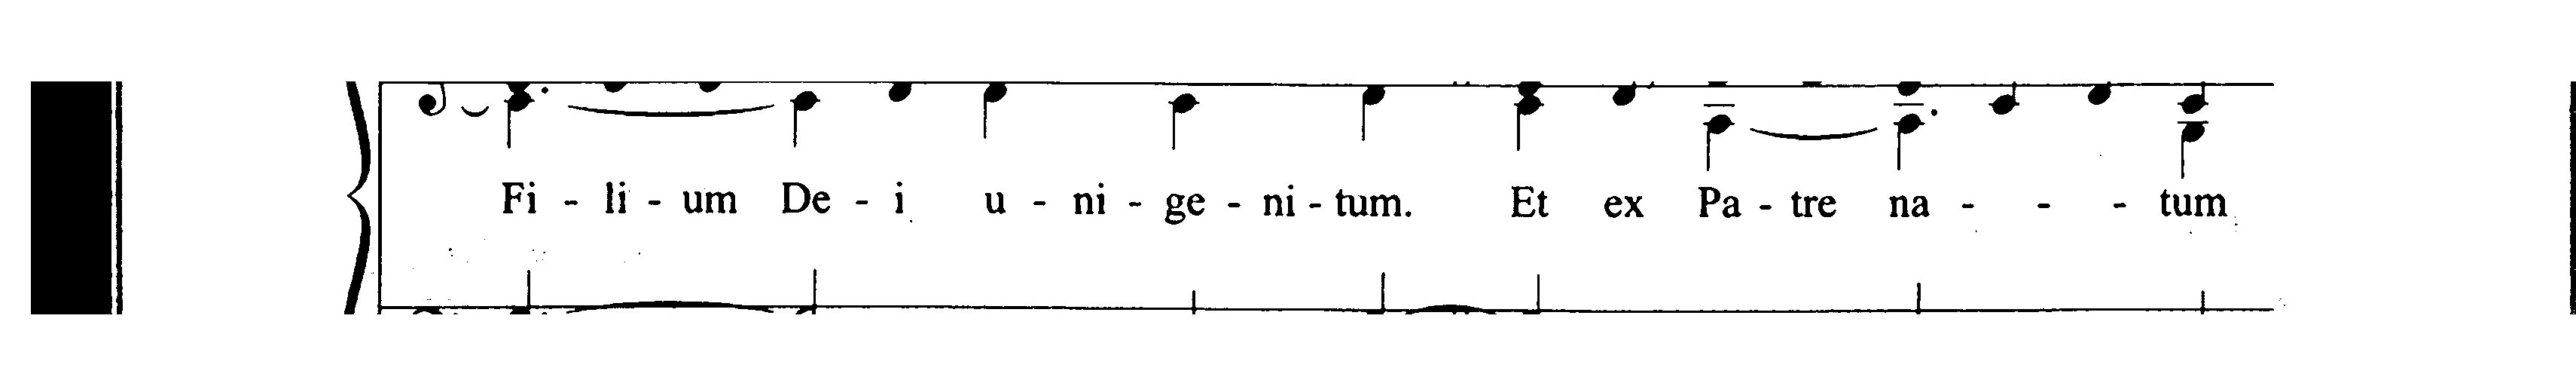
\includegraphics[width = 16.5cm, frame] {image//exampleImage//r_001.png} 
			        \end{center}
			        \caption
        			    [Przykładowy obraz z którego rozpoznawany jest tekst.]  
        			    {Przykładowy obraz z którego rozpoznawany jest tekst.}  
        			    \label{fig:exImgRead01}
	        \end{figure}\\
	        Tekst rozpoznany na podstawie Rysunku \ref{fig:exImgRead01}: 
	        " ł vrfrZżrvrwrjFiliumDeiuni—genitumEtexPatrenatum        u g i  DP  ".
	        \begin{figure}[!ht]  
			        \begin{center}
				        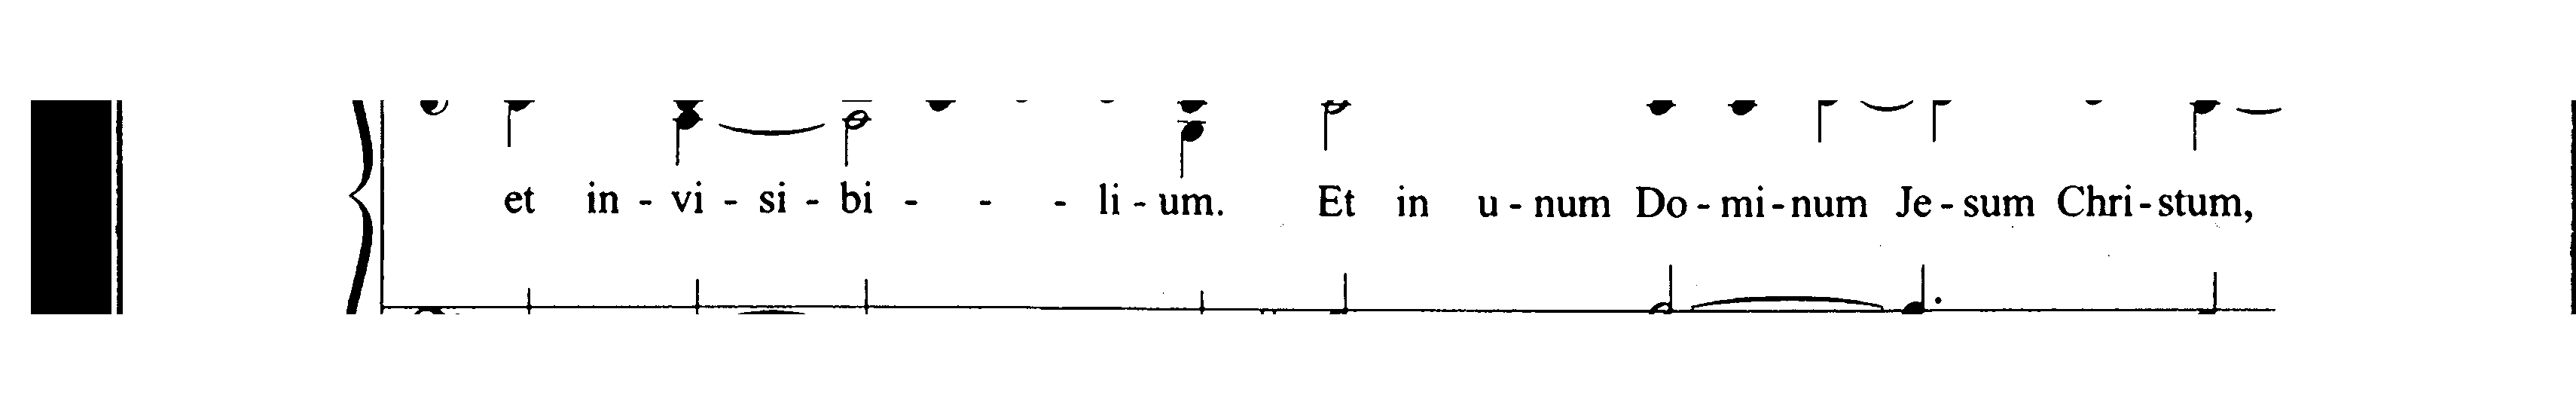
\includegraphics[width = 16.5cm, frame] {image//exampleImage//r_002.png} 
			        \end{center}
			        \caption
        			    [Przykładowy obraz z którego rozpoznawany jest tekst.]  
        			    {Przykładowy obraz z którego rozpoznawany jest tekst.}  
        			    \label{fig:exImgRead02}
	        \end{figure}\\
	        Tekst rozpoznany na podstawie Rysunku \ref{fig:exImgRead02}: 
	        " l v”Ietinv1«Ivetin vi Vsira~bii—il IA  ;rrvrrliumEtinunumDominumJesumChristun1L=L4L›L  i   FEiii›—wII  numDo~~minumA ii „Il mJe s lllC ri FSii ".
	        \begin{figure}[!ht]  
			        \begin{center}
				        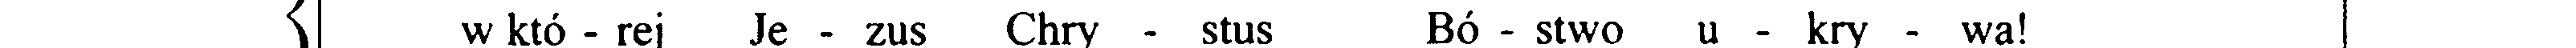
\includegraphics[width = 16.5cm, frame] {image//exampleImage//r_003.png} 
			        \end{center}
			        \caption
        			    [Przykładowy obraz z którego rozpoznawany jest tekst.]  
        			    {Przykładowy obraz z którego rozpoznawany jest tekst.}  
        			    \label{fig:exImgRead03}
	        \end{figure}\\
	        Tekst rozpoznany na podstawie Rysunku \ref{fig:exImgRead03}: 
	        " Wktó reiJe ZusChIV st s ó FStW O  kIV Wa   ".
	        \begin{figure}[!ht]  
			        \begin{center}
				        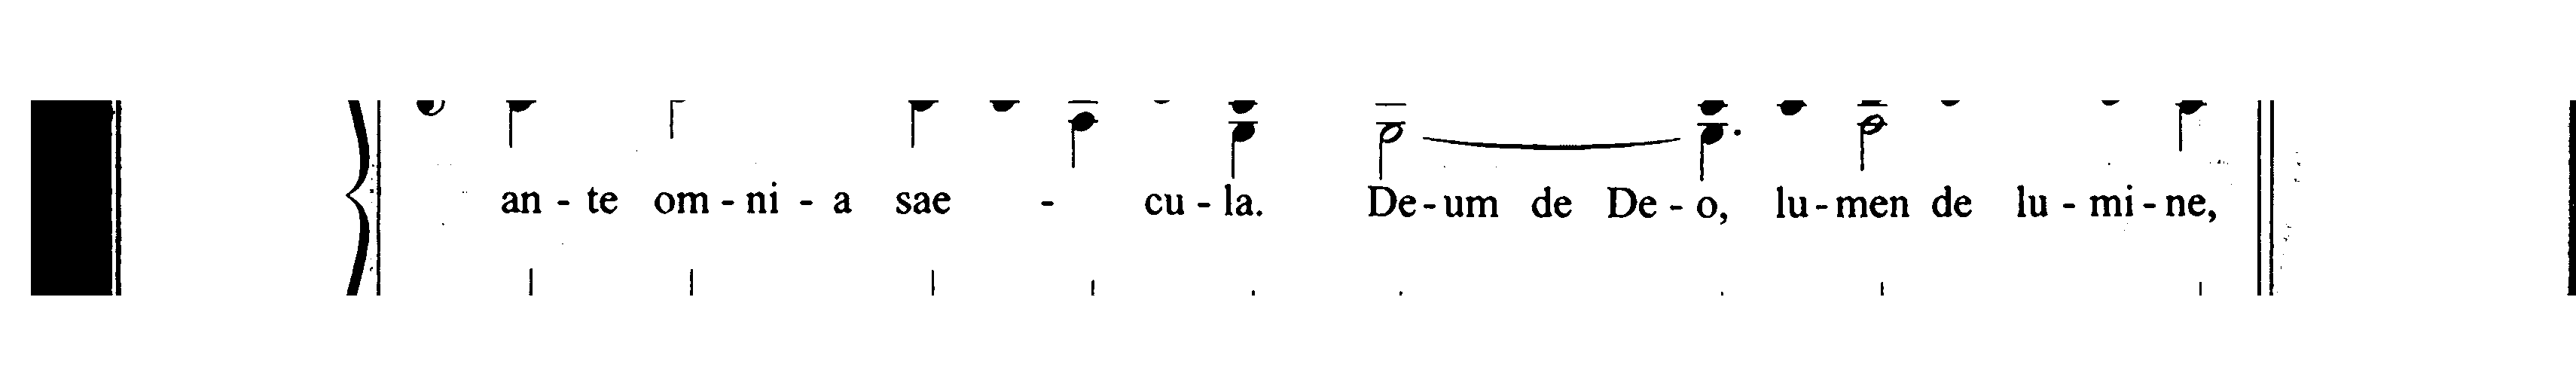
\includegraphics[width = 16.5cm, frame] {image//exampleImage//r_004.png} 
			        \end{center}
			        \caption
        			    [Przykładowy obraz z którego rozpoznawany jest tekst.]  
        			    {Przykładowy obraz z którego rozpoznawany jest tekst.}  
        			    \label{fig:exImgRead04}
	        \end{figure}\\
	        Tekst rozpoznany na podstawie Rysunku \ref{fig:exImgRead04}: 
	        "    TĘrI teIo   iii F5rSCI LA   CU la De   ~hmdeDeFJ   lu  „ll»de      i lLŚ     ".
	        
	        Na podstawie powyższych przykładów można zauważyć, że rozpoznawanie tekstu jest zagadnieniem nietrywialnym, złożonym. W wychwyconych tekstach można zidentyfikować poszczególne wyrazy i frazy (teksty rozpoznany na podstawie Rysunków \ref{fig:exImgRead01}, \ref{fig:exImgRead02}, \ref{fig:exImgRead03}). Idealne przykłady detekcji linii w których znajduje się tekst (Rysunek \ref{fig:exImgRead03}) niekoniecznie dają idealne wyniki, jest to spowodowane niedoskonałym algorytmem klasyfikującym poprawnie wycięte z obrazu litery. Zaś jeśli rozpoznana linia zwierająca tekst zawiera dodatkowo nie wycięte znaki muzyczne to mają one wpływ na dalsze przetwarzanie obrazu (wycięcie liter), a w efekcie na rozpoznany tekst (tekst rozpoznany na podstawie Rysunku \ref{fig:exImgRead04}).
	        
        \subsection{Graficzny interfejs użytkownika}
	        \begin{figure}[h!]
                \centering
                \begin{subfigure}[b]{0.47\linewidth}
                    \includegraphics[width=\linewidth]{image//gui//app001.png}
					\caption{}
                \end{subfigure}
                \begin{subfigure}[b]{0.47\linewidth}
                     \includegraphics[width=\linewidth]{image//gui//app002.png}
					\caption{}
                \end{subfigure}
                \newline
                
				\begin{subfigure}[b]{0.47\linewidth}
                    \includegraphics[width=\linewidth]{image//gui//app003.png}
					\caption{}
                \end{subfigure}
                \begin{subfigure}[b]{0.47\linewidth}
                    \includegraphics[width=\linewidth]{image//gui//app004.png}
					\caption{}
                \end{subfigure}
                \caption
                    [GUI]
					{GUI}
					\label{fig:gui}
            \end{figure}
            
             Wszystkie opracowane rozwiązania zostały udostępnione poprzez prosty graficzny interfejs użytkownika. Po uruchomieniu programu pojawia się okienko (Rysunek \ref{fig:gui} (a)), następnie  użytkownik określa kilka parametrów, które wykorzystują algorytmy (czy dodatkowo ma być usunięty czarny obszar po lewej stronie, czy tekst znajduje się pomiędzy dwoma liniami muzycznymi czy pod linią muzyczną). Kolejnym krokiem jest wybór pliku z zasobów komputera, (Rysunek \ref{fig:gui} (b)). Teraz wybrany plik zostaje przetworzony przez wszystkie wcześniej opisane algorytmy. Okienko wyświetla informację jaki algorytm został wykonany i zmienia się niebieski pasek postępu. Gdy zdjęcie przejdzie przez wszystkie algorytmy pasek postępu osiąga wartość maksymalną i zostaje wyświetlona ścieżka do wyjściowych plików .txt.
	        
	   \newpage  
	   \section{Podsumowanie}
	   \hspace{\spacingIndent} W niniejszej pracy dyplomowej zostały zrealizowane główne jej założenia. Opracowane algorytmy umożliwiają pozyskanie tekstu ze stron zawierających znaki muzyczne. Wśród uzyskanego tekstu możemy odnaleźć poszczególne sylaby, a nie rzadko i wyrazy. Identyfikacją liter składających się na poszczególne wyrazy może zostać jeszcze polepszona, przede wszystkim przez wykorzystanie dokładniejszych algorytmów wycinających poszczególne litery, powiększenie zbioru liter (majuskuł, minuskuł) i linii (tekstu, pięciolinii) na których uczą się sieci neuronowe. Dzięki zastosowaniu sztucznej inteligencji opracowane algorytmy są bardziej uniwersalne i umożliwią pracę ze znacząca liczbą powszechnie wykorzystywanych śpiewników wpisujących się w następujące dwa schematy [pięciolinia tekst pięciolinia], [pięciolinia tekst]. Dzięki wytworzeniu oprogramowania zgodnie z zasadami programowania zorientowanego obiektowo, z łatwością możemy do powyższych dwóch struktur dodawać kolejne w różnych konfiguracjach na przykład [pięciolinia tekst pięciolinia pięciolinia].
	   
	   Kolejnym z celów pracy, który został zrealizowany to budowa graficznego interfejsu użytkownika, wybrana technologia i architektura systemu umożliwiła dość proste przejście z aplikacji konsolowej do aplikacji posiadającej prosty interfejs graficzny. Aplikacja może, a nawet powinna być rozwijana również w kierunku budowy bardziej rozbudowanego GUI, umożliwiającego użytkownikowi dobór parametrów (dla algorytmów) dla wybranego pliku poprzez udostępnienie rezultatów poszczególnych algorytmów w czasie rzeczywistym.
	   
	   Dzięki pracy nad budową aplikacji mogłem rozwinąć swoje zdolności algorytmiczne i programistyczne. Zapoznanie się z podstawami teoretycznymi systemów przetwarzających tekst, działania sztucznych sieci neuronowych, algorytmów przetwarzających obrazy oraz z narzędziami związanymi z tymi zagadnieniami -- Tesseract, OpenCV, DL4J pozwoliło autorowi na zdobycie i rozwój swojej wiedzy i umiejętności.
	   
	   Horyzont zastosowań sztucznej inteligencji nieustannie odkrywa przed osobami zajmującymi się tym zagadnieniem nowe wody. Na przestrzeni lat wąskie przeznaczenie sztucznej inteligencji znacząco się zwiększyło i dziś znajduje użytek w wielu dziedzinach życia. Taki wzrost znaczenia sztucznej inteligencji pociąga za sobą wzrostu zapotrzebowania na specjalistów zajmujących się uczeniem maszynowy. Dzisiejszy rynek pracy bardzo ceni i poszukuje takich osób. Zagadnienia poruszane przeze mnie w pracy dyplomowej niewątpliwie będą stanowiły cenna umiejętność podczas poszukiwań przyszłej pracy zawodowej. 
	   
	   
	   
	   \newpage

        \addtocontents{toc}{\protect\setcounter{tocdepth}{1}}
        \section{Bibliografia}
        \begin{thebibliography}{99}
            \subsection{Źródła książkowe:}
            \bibitem{1} 
            Rączkowski F., \textit{Śpiewajmy Bogu}, Płock, Hejnał, 2012
 
            \bibitem{2} 
            Siedlecki J., \textit{Śpiewnik kościelny}, Wyd. XL (poprawione), Kraków,
            Instytut Teologiczny Księży Misjonarzy, 2011.
        
            \bibitem{3} 
            Kaehler A., Bradski G., OpenCV 3. \textit{Komputerowe rozpozn1awanie obrazu w C++ przy użyciu biblioteki OpenCV}, Gliwice, Helion, 2017.
            
            \bibitem{4} 
            Shanmugamani R., \textit{Deep Learning for Computer Vision}, Birmingham, Packt Publishing, 2018

            \subsection{Źródła internetowe:}
            Data dostępu 2018.07.15
            \bibitem{5} 
            \href{https://opencv.org}{\url{https://opencv.org}}.
            
            \bibitem{6}    
            \href{https://docs.opencv.org//3.1.0//index.html}{\url{https://docs.opencv.org//3.1.0//index.html}}.
            
            \bibitem{7}
            \href{https://docs.opencv.org//java//3.1.0}{\url{https://docs.opencv.org//java//3.1.0}}.
            
            \bibitem{8}    
            \href{http://tess4j.sourceforge.net}{\url{http://tess4j.sourceforge.net}}.
            
            \bibitem{9}    
            \href{https://deeplearning4j.org//index.html}{\url{https://deeplearning4j.org//index.html}}.
            
            \bibitem{10}
            \href{https://nd4j.org//doc}{\url{https://nd4j.org//doc}}.
            
            \bibitem{11}
            \href{https://depiesml.wordpress.com//category//deeplearning4j}{\url{https://depiesml.wordpress.com//category//deeplearning4j}}.
    
            \bibitem{12}
            \href{https://ksopyla.com//python//operacja-splotu-przetwarzanie-obrazow}{\url{https://ksopyla.com//python//operacja-splotu-przetwarzanie-obrazow}}.
                
            \bibitem{13}    
            \href{https://github.com//Kulbear//deep-learning-nano-foundation//wiki//ReLU-and-Softmax-Activation-Functions}{\url{https://github.com//Kulbear//deep-learning-nano-foundation//wiki}}.
            %https://github.com/Kulbear/deep-learning-nano-foundation/wiki/ReLU-and-Softmax-Activation-Functions
    
            \bibitem{14}
            \href{http://www.szkolazpasja.pl//rastrowa}{\url{http://www.szkolazpasja.pl//rastrowa}}.
            
            \bibitem{15}  \href{https://leonardoaraujosantos.gitbooks.io//artificial-inteligence//content//dropout_layer.html}{\url{https://leonardoaraujosantos.gitbooks.io//artificial-inteligence//content//dropout_layer.html}}.
                
            \bibitem{16}    
            \href{https://www.tiobe.com//tiobe-index}{\url{https://www.tiobe.com//tiobe-index}}.
        \end{thebibliography}
	        \includepdf[pages=-]{include.pdf}
\end{document}